\section{Flight Experiment}
\label{sec:experiment}

In addition to the simulation study in Section \ref{sec:simulation}, the quadrotor system was tested by experiments to evaluate the nonlinear controller. The flight experiments were executed at the motion capture arena of the Intelligent Robotics Laboratory(IRL) at the University of Illinois at Urbana-Champaign \cite{irl}. The quadrotor was controlled with the outer-loop and inner-loop control stated in Chapter \ref{ch:control_system}. The linear attitude control stated in Section \ref{sec:pid} was also tested with the outer-loop control of Section \ref{sec:outer_loop} to compare with the performance of the nonlinear attitude control. The motion of the quadrotor is recorded by a motion capture system. 
In this chapter, the experimental setup for the evaluation of the quadrotor is stated, and then, the experiment results and discussion about them are followed.

\subsection{Motion Capture Arena}

The quadrotor experiments were done at IRL's motion capture arena for human safety. The arena is equipped with safety facilities for UAVs' flight experiments. The arena is isolated so that the quadrotor does not damage anything out of the arena. In order to limit the range of quadrotors' maneuver and protect them from potential damage, the arena is surrounded by nets. In addition, the floor of the arena is covered with shock absorbing foams to protect the quadrotor from damaging itself. With the setup, potential accidents from the quadrotor's malfunction can be prevented.

Mounted on the ceiling of the four conners of the room, there are installed two motion capture camera; in total eight cameras consists of the motion capture system. The whole arena area is covered by the motion capture range, and the motion capture system measures motion of the object that has reflective motion capture markers on it.

\begin{figure}
    \centering
    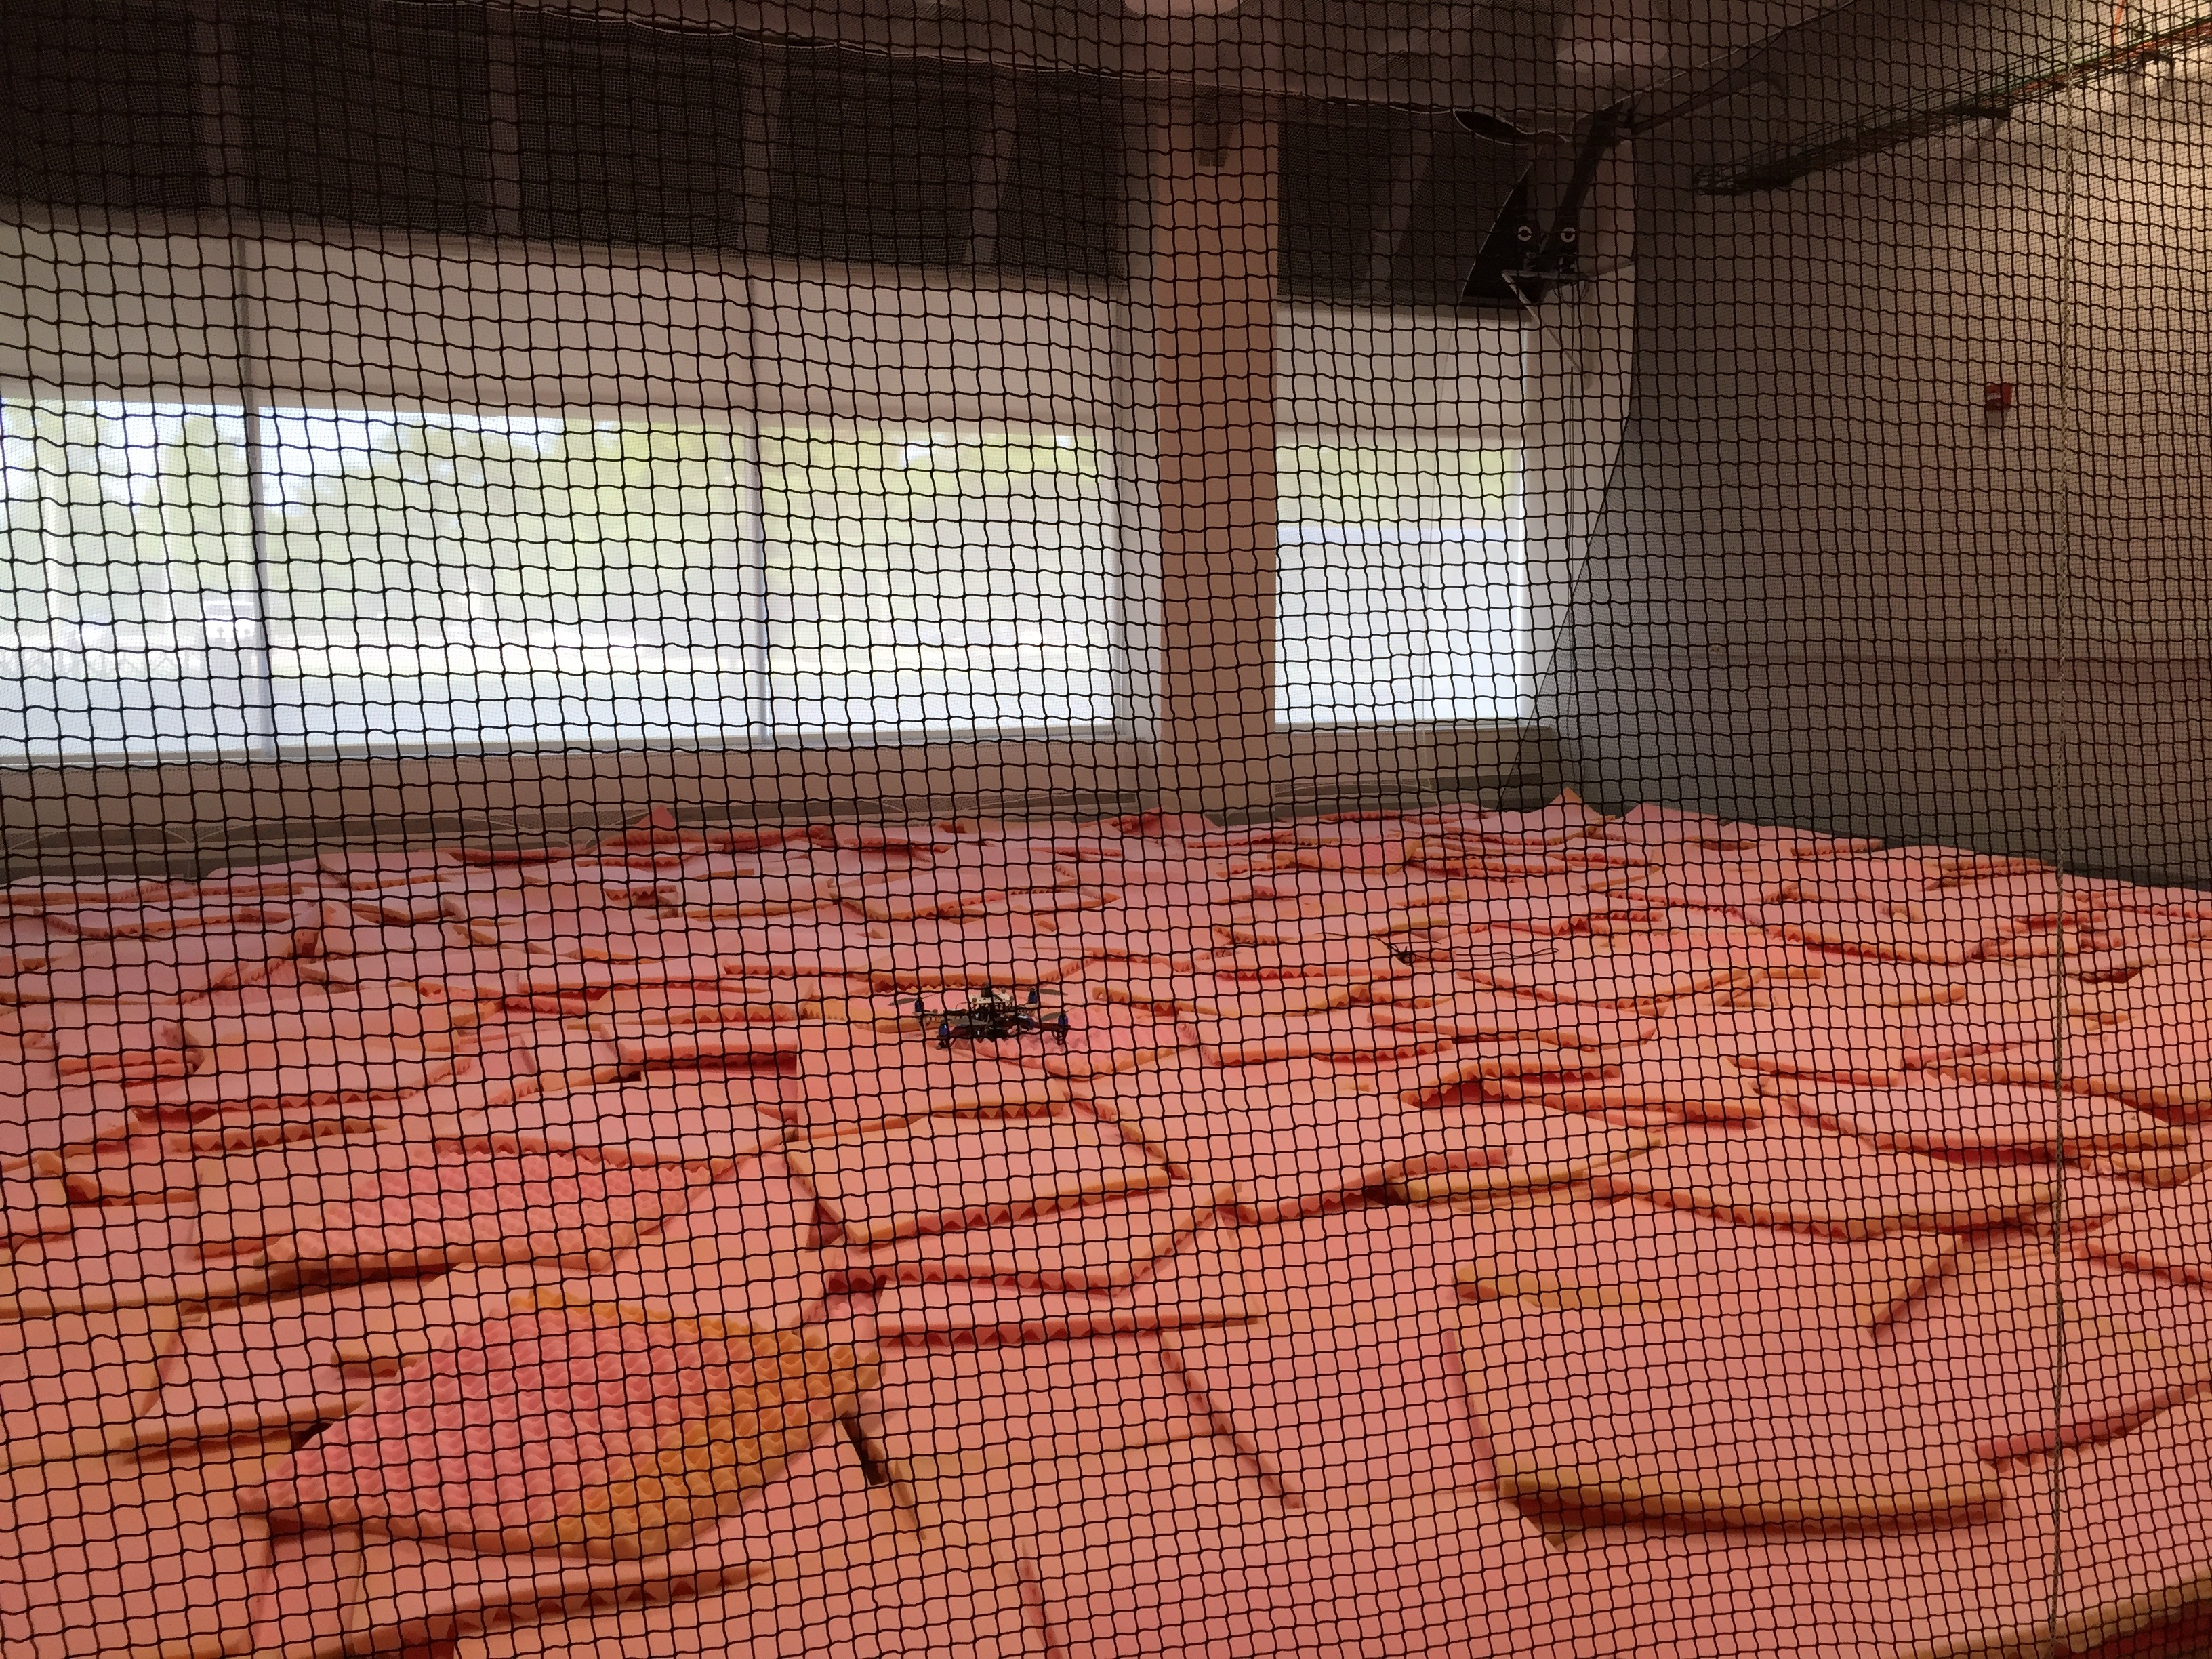
\includegraphics[width=0.8\textwidth]{graphics/arena.jpg}
    \caption{Motion Capture Arena of the Intelligent Robotics Laboratory}
    \label{fig:arena}
\end{figure}

\subsection{Motion Capture System}
IRL's motion capture system consists of 8 Vicon T-series T40S Cameras mounted around the arena. Motion capture cameras of Vicon radiate infrared rays and capture infrared rays reflected from the markers. By synchronizing the pixel coordinate of the reflective markers at multiple motion capture cameras, the motion capture system obtains the position information of the markers \cite{vicon}.

\begin{figure}
    \centering
    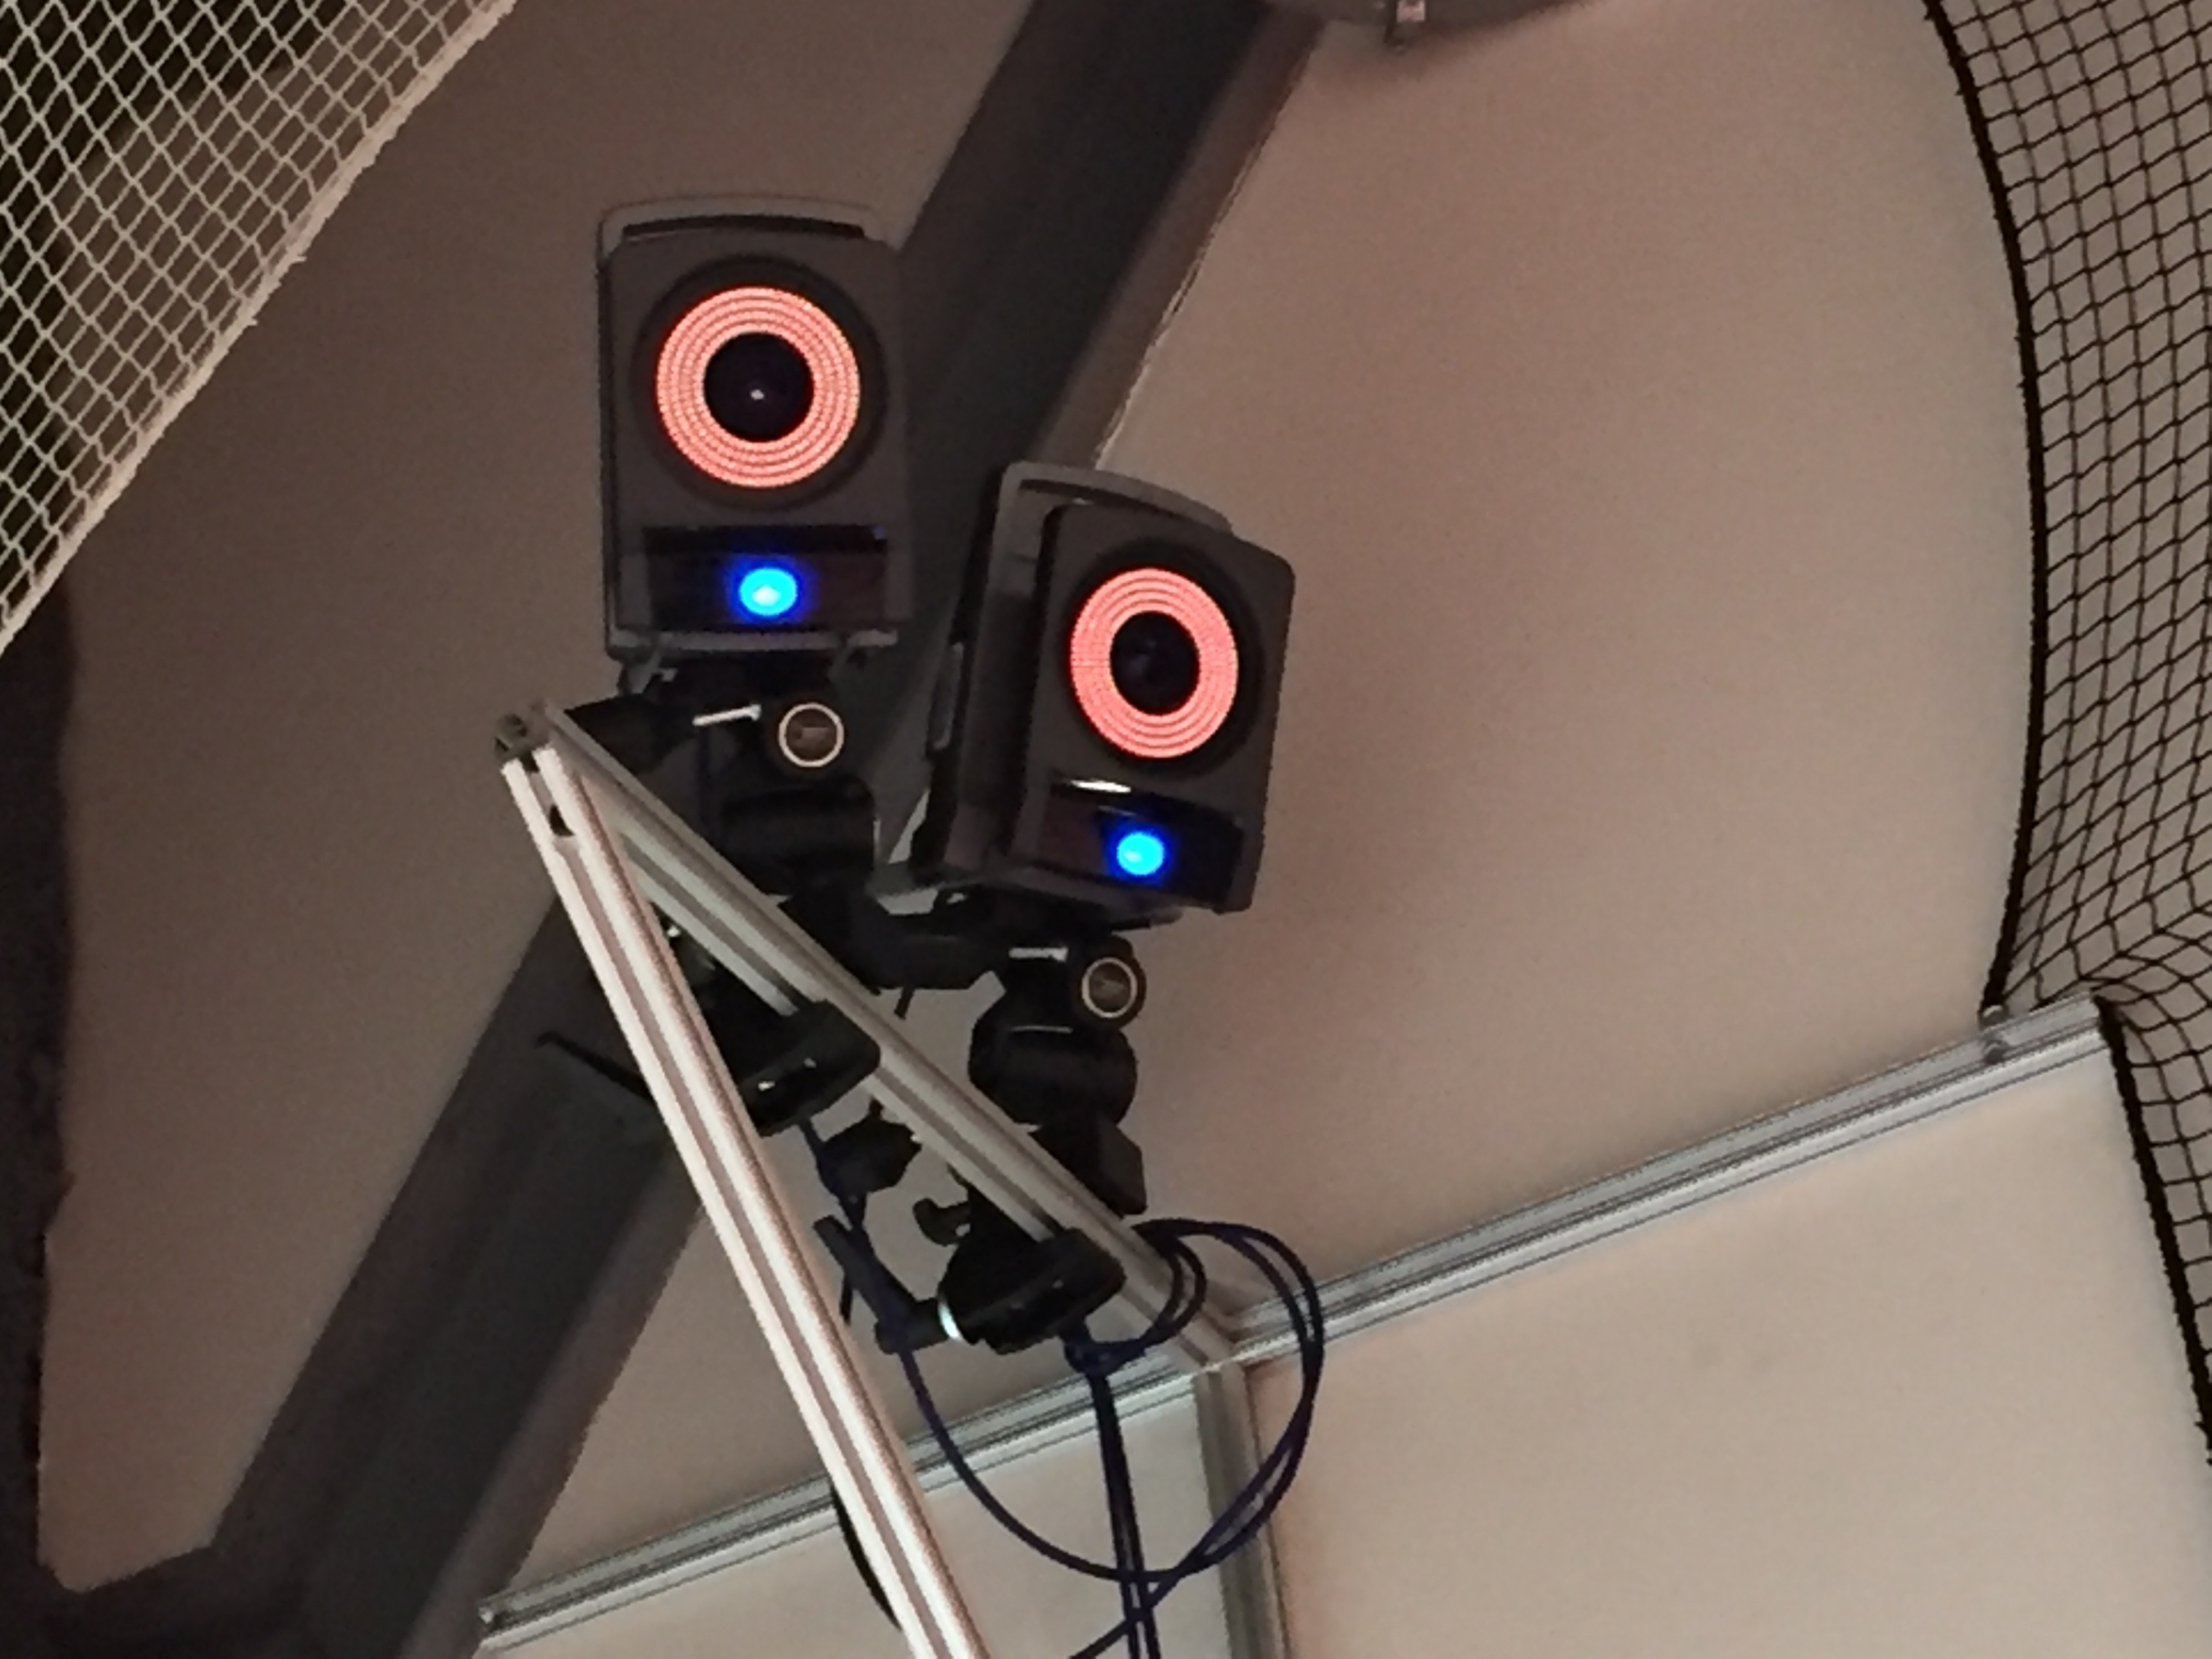
\includegraphics[width=0.5\textwidth]{graphics/vicon_camera.jpg}
    \caption{Vicon Motion Capture Cameras}
    \label{fig:arena}
\end{figure}

Prior to the experiment, it is necessary to register an object that is a rigid body and has multiple markers on it. Then, the motion capture system saves the geometric information of the reflective markers in the database and recognizes the object. In order to measure both the position and attitude of the quadrotor, at least 3 reflector markers must be located on the quadrotor since a plane consist of at least three points. In this experiment, 7 markers are fixed on the quadrotor to guarantee the precision of the motion information; three are located on the quadrotor's legs and the other markers are stick on the top of the quadrotor. To avoid incorrect measurement of the quadrotor's attitude, the markers are installed asymmetrically.

The motion capture system of IRL works with Tracker, a graphic user interface software for Vicon, and Vicon Bridge, a ROS package developed by the autonomous systems laboratory at ETH Zurich are used for streaming the data of the quadrotor position and attitude.

\begin{figure}
    \centering
    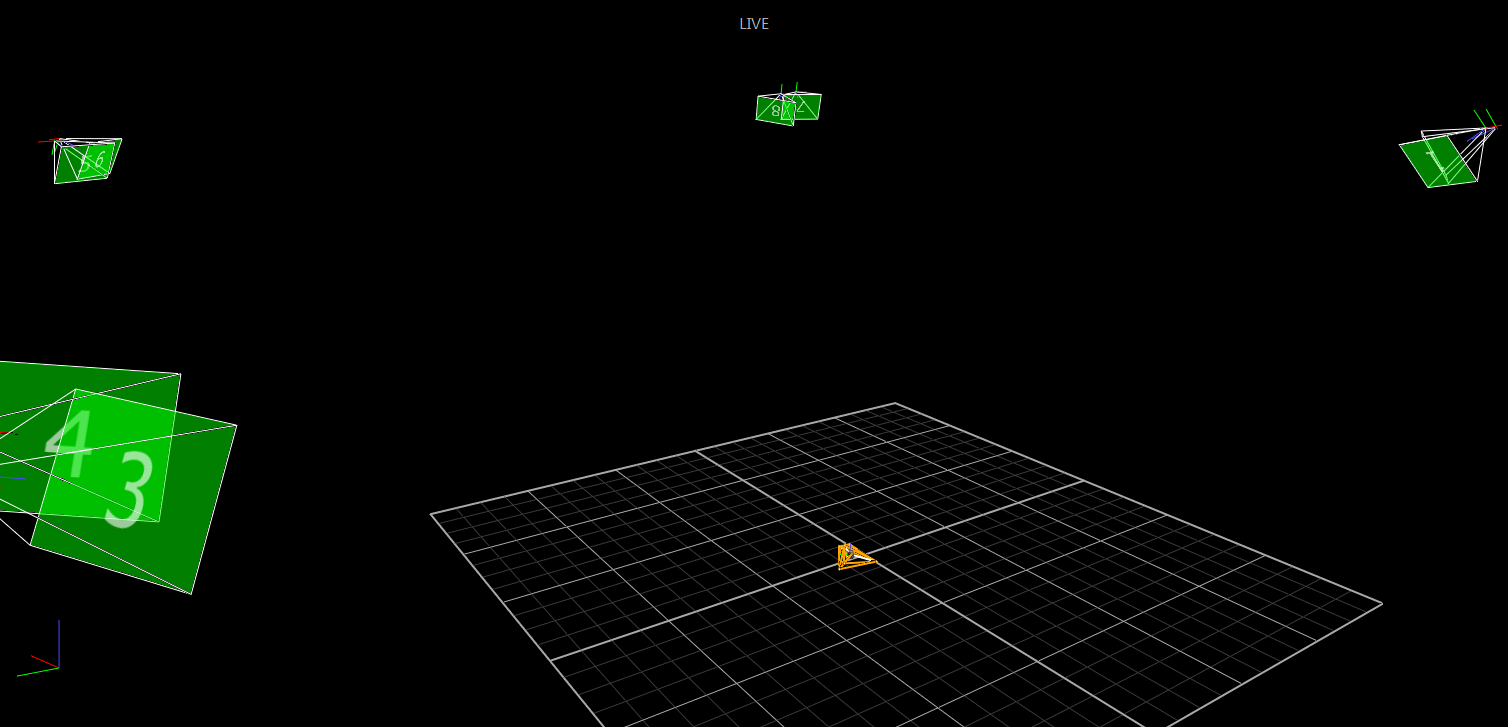
\includegraphics[width=0.8\textwidth]{graphics/tracker.png}
    \caption{Vicon Motion Capture Interface}
    \label{fig:arena}
\end{figure}

\subsection{Experiment Setup}

Prior to experiment, we tuned the control gains of the nonlinear and linear inner-loop controllers, based on the simulated control gains in Section \ref{sec:simulation} and adjusted the gains by multiple flight tests.

In the experiments, the quadrotor was controlled by the PID outer-loop controller described in Section \ref{sec:outer_loop} and either the nonlinear attitude control of Chapter \ref{ch:control_system} or the linear attitude control of Section \ref{sec:pid}. Since it is difficult to set the same desired state of the quadrotor for its position, the position and attitude trajectories for the quadrotor to reach the desired position are used to evaluate performance of each inner-loop controller. Therefore, the desired position of each flight experiment is set to be as far as possible in the motion capture arena from the initial position. The  outer-loop control of the x, y-axis directions is expected to drift since the quadrotor does not include internal position measurement for x, y-axis directions.

The quadrotor's experiments were conducted with focus on control system's stability and agility. First, in order to evaluate the quadrotor's stability, we changed the altitude of the waypoint from 1.8 m to 3 m. The quadrotor first would hover, stabilize its position at the first waypoint, moves to the next waypoint, and land. To evaluate roll agility, we changed the waypoint to either left side or right side from the first waypoint, and then control the quadrotor to land. The waypoint was changed to either forward or backward to validate pitch agility. Finally, yaw performance was also tested by setting desired yaw to be \( \pm {{\pi}\over{2}}\) while the quadrotor hovering on the waypoint. Similarly, as yaw converges to the desired yaw, the quadrotor landed. To summarize, the follow cases were tested.
\begin{enumerate}
\item Take off, change altitude from 1.8m to 3.0m, and land.
\item Take off, move right side, and land.
\item Take off, move left side, and land.
\item Take off, move forward, and land.
\item Take off, move backward, and land.
\item Take off, turn \( \pm {{\pi}\over2}\) to the right, and land.
\item Take off, turn \( \pm {{\pi}\over2}\) to the left, and land.
\end{enumerate}


\subsection{Experiment Results}
All the experimental data are filtered by a low-pass filter and transformed into the coordinate system that is defined in the motion capture system. Also the origin point of each case is defined to be the initial position of the quadrotor. The trajectories and attitude changes over time are plotted in Figures \ref{fig:exp_alt} - \ref{fig:exp_yaw_minus}. Full lines represent the quadrotor's actual trajectories and dashed lines represent the desired position or waypoints.

\begin{figure}
    \centering
    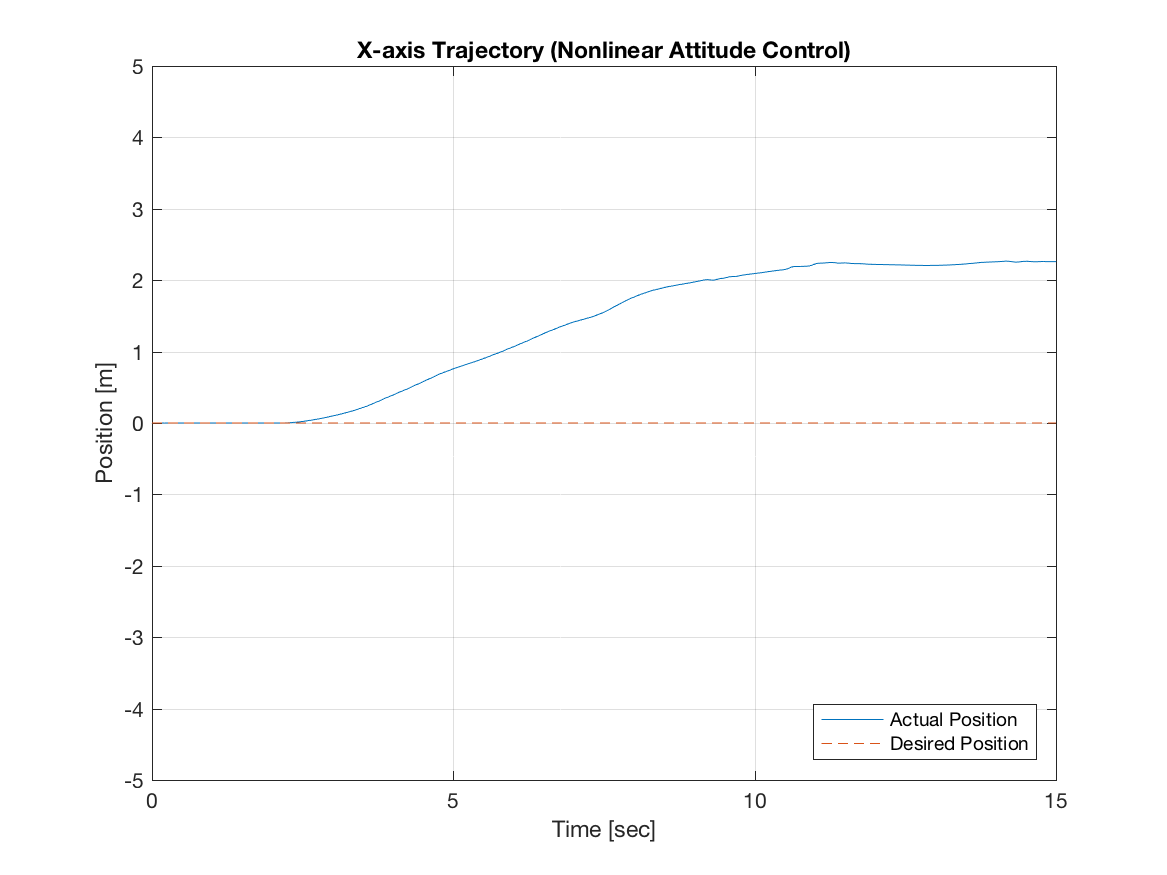
\includegraphics[width=0.45\textwidth]{graphics/experiment_plots/altitude_non_position_x.png}
    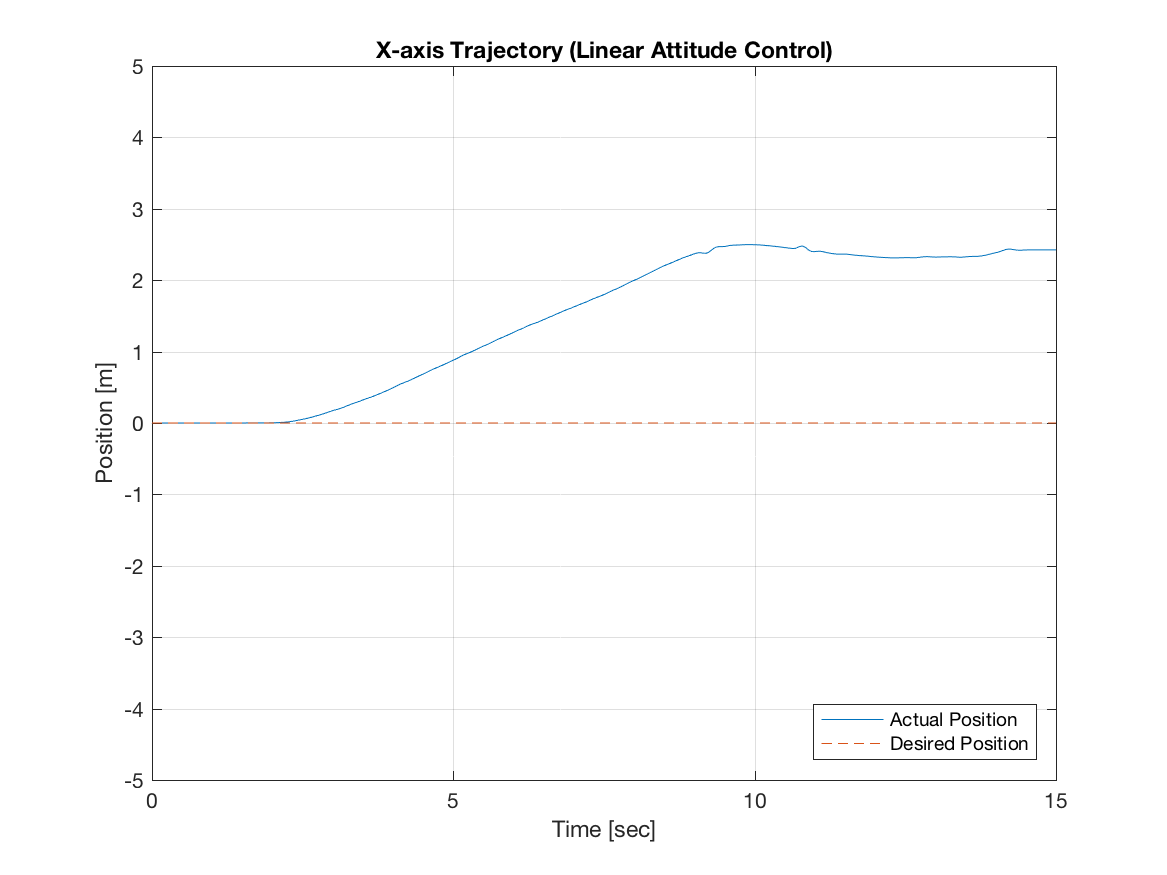
\includegraphics[width=0.45\textwidth]{graphics/experiment_plots/altitude_pid_position_x.png}
    
    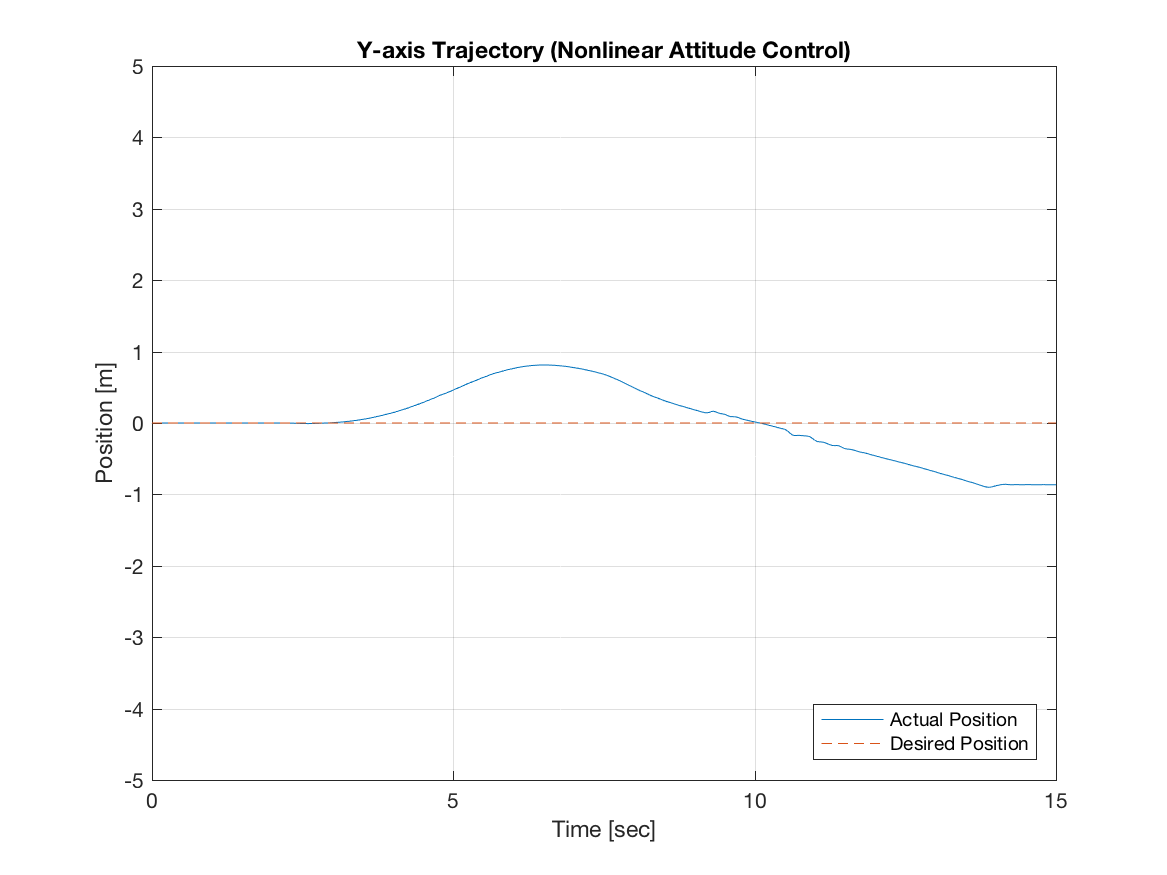
\includegraphics[width=0.45\textwidth]{graphics/experiment_plots/altitude_non_position_y.png}
    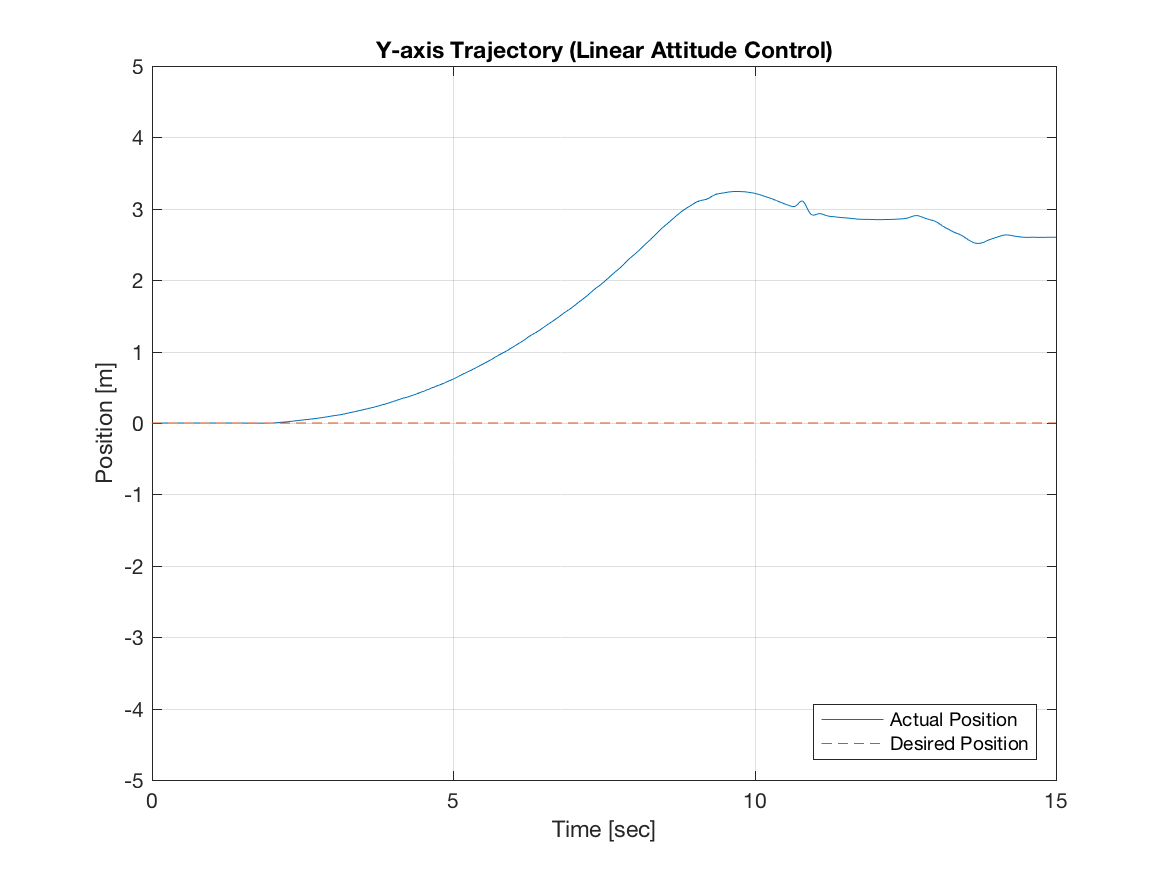
\includegraphics[width=0.45\textwidth]{graphics/experiment_plots/altitude_pid_position_y.png}
    
    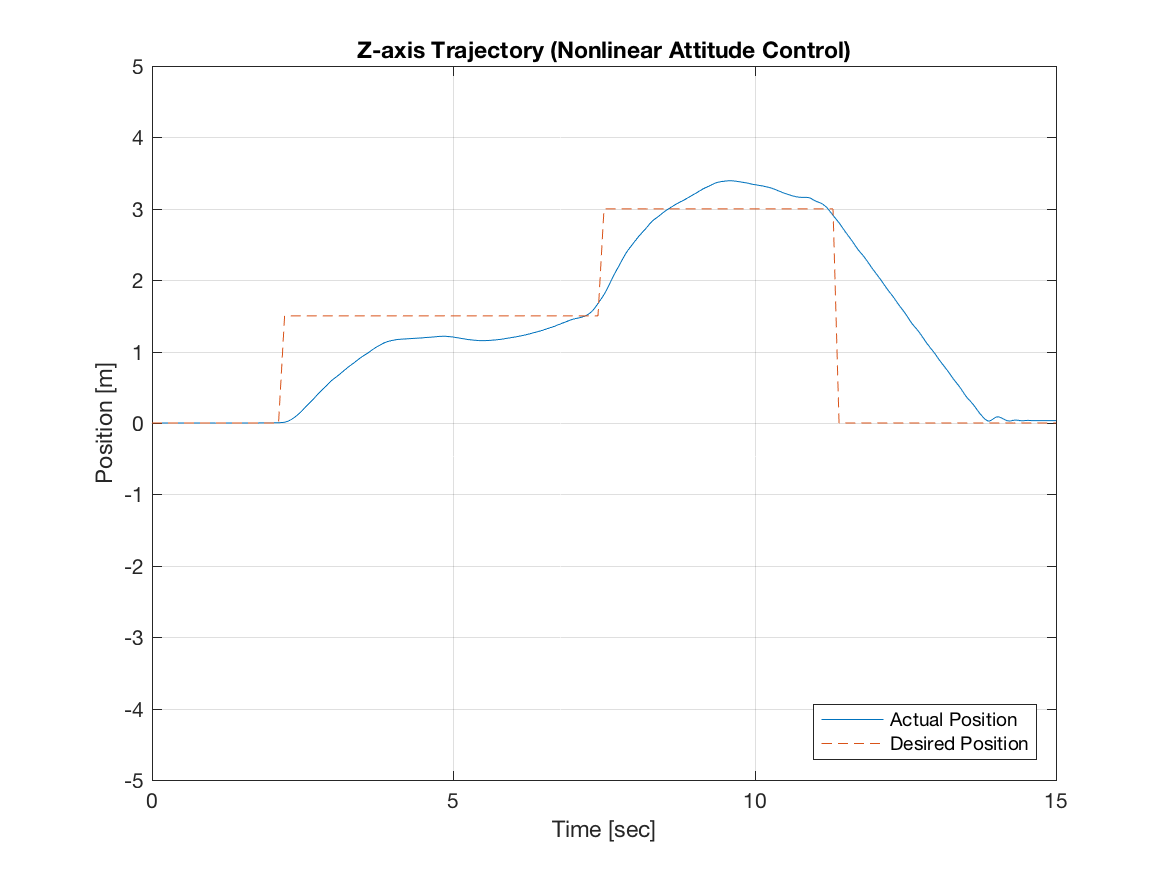
\includegraphics[width=0.45\textwidth]{graphics/experiment_plots/altitude_non_position_z.png}
    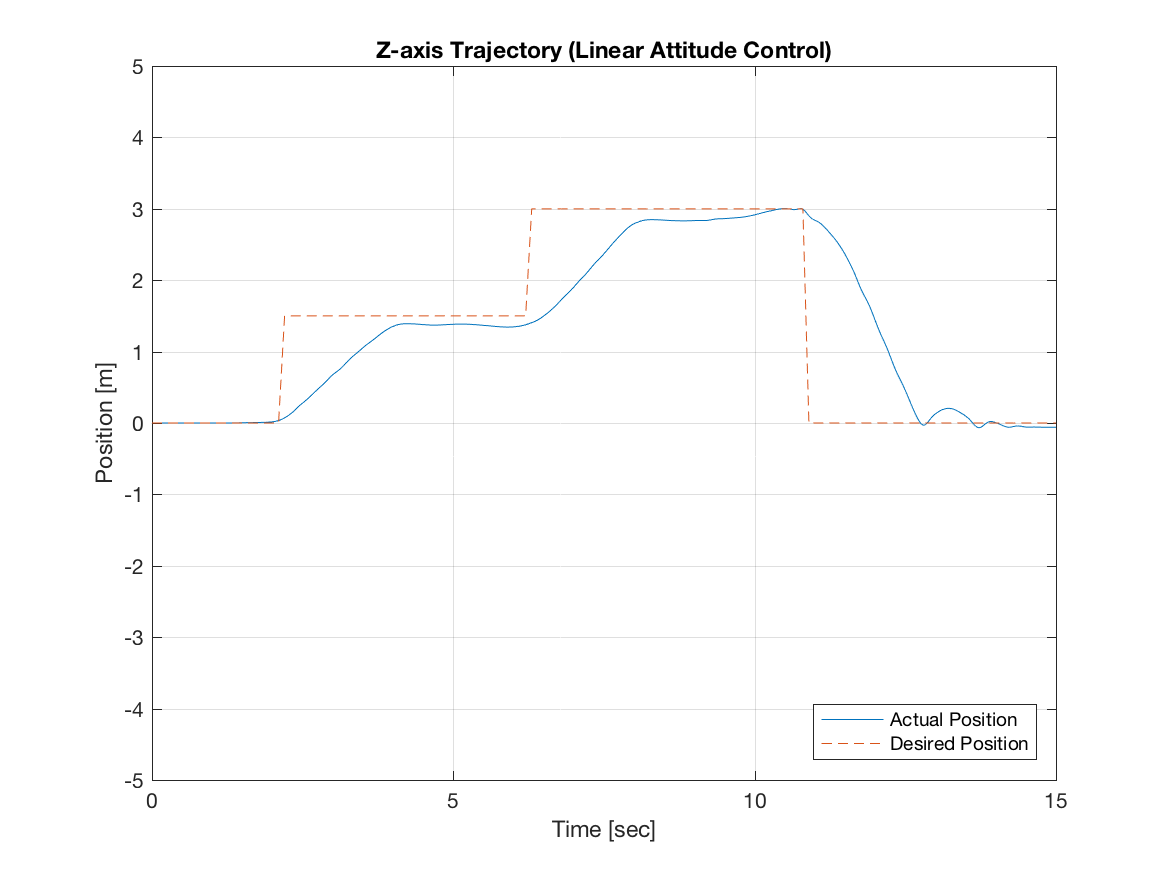
\includegraphics[width=0.45\textwidth]{graphics/experiment_plots/altitude_pid_position_z.png}

    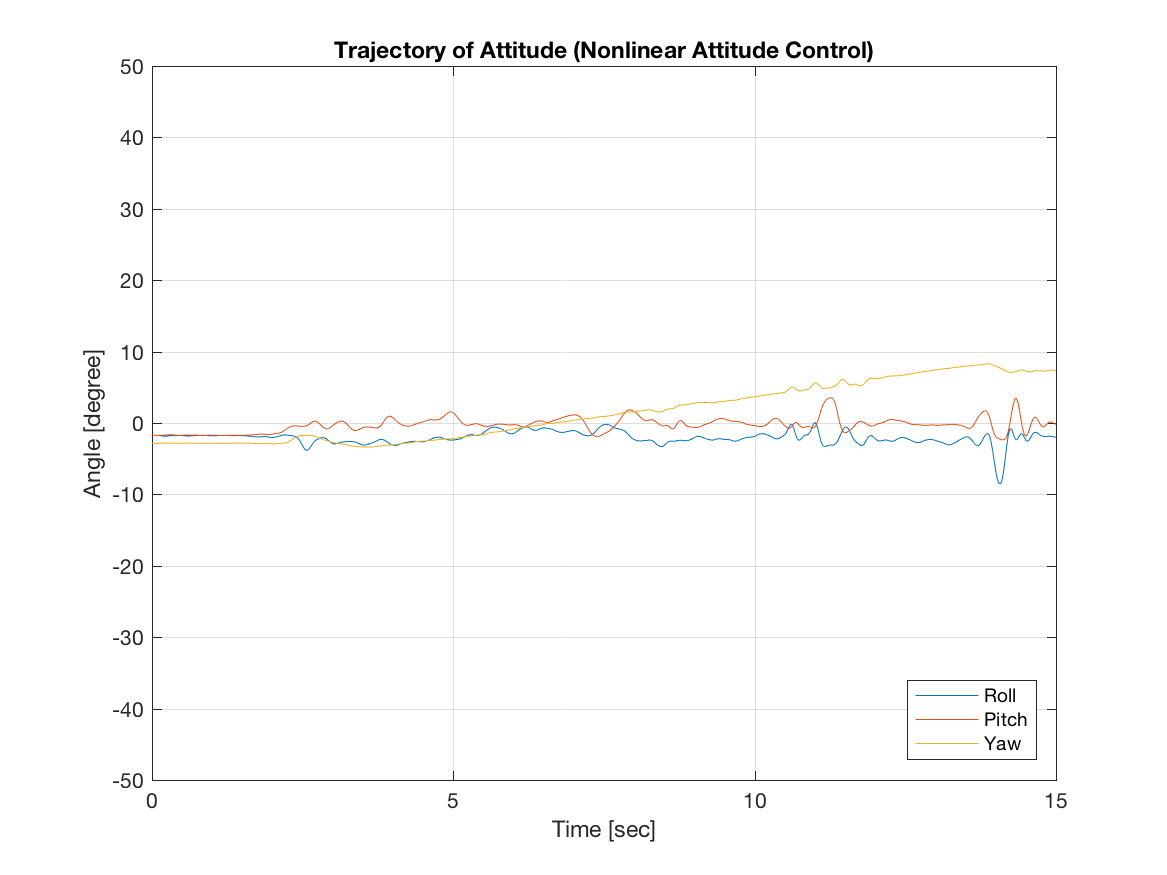
\includegraphics[width=0.45\textwidth]{graphics/experiment_plots/altitude_non_attitude.png}
    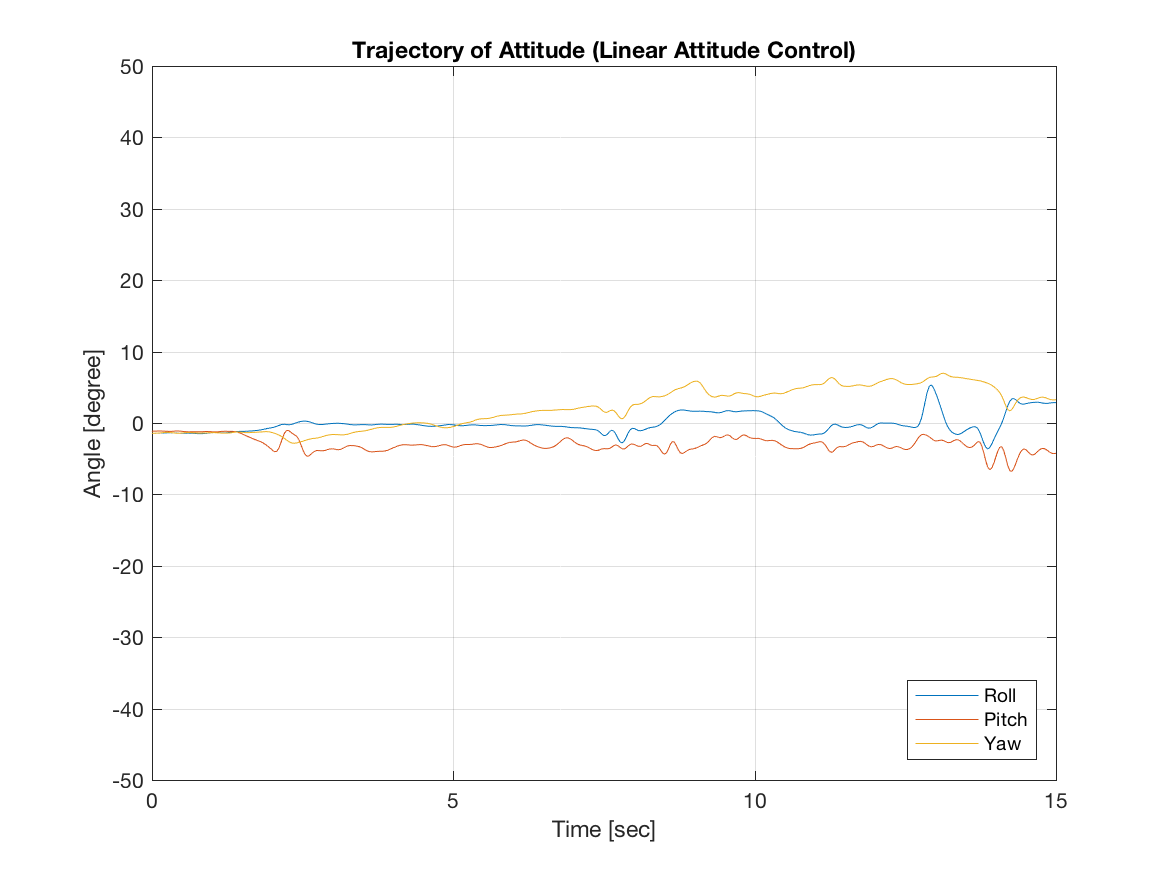
\includegraphics[width=0.45\textwidth]{graphics/experiment_plots/altitude_pid_attitude.png}
    \caption{Experiment Result (Case 1)}
    \label{fig:exp_alt}
\end{figure}

\begin{figure}
    \centering
    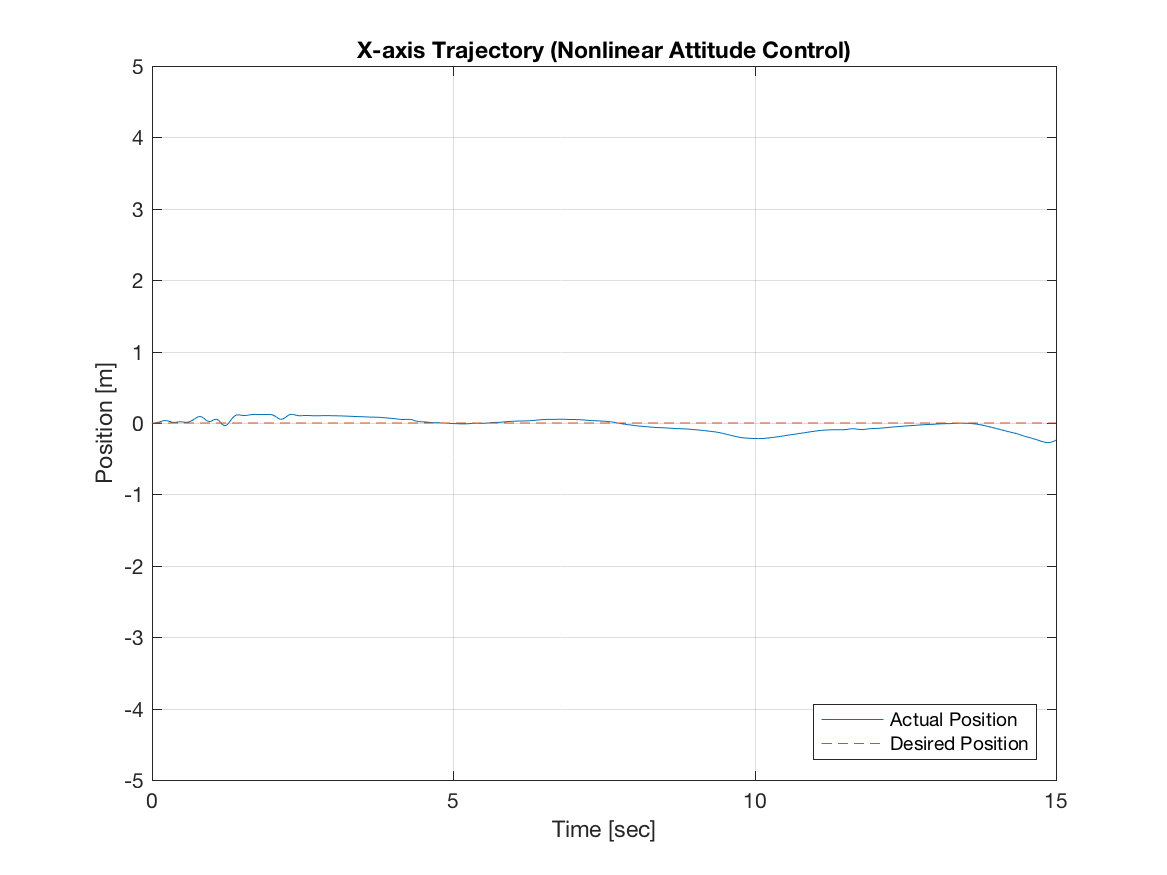
\includegraphics[width=0.45\textwidth]{graphics/experiment_plots/roll_plus_non_position_x.png}
    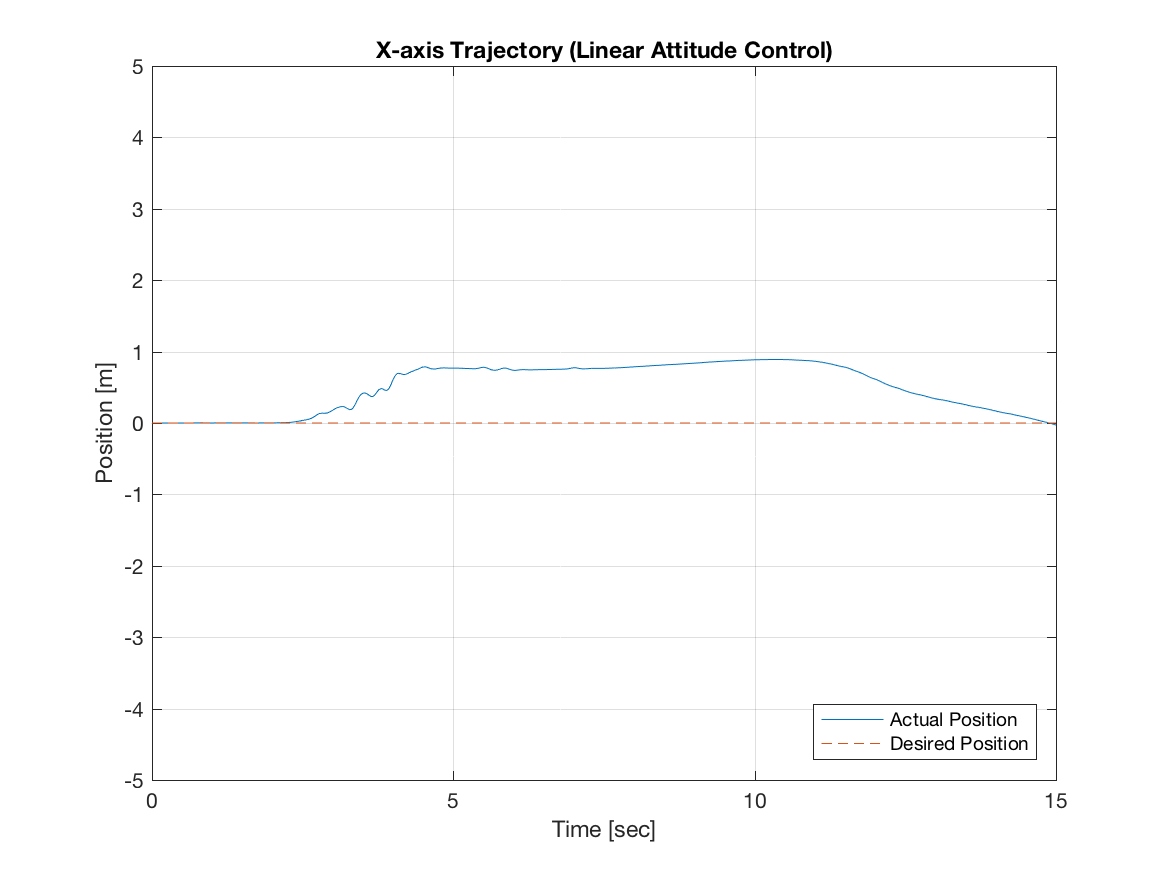
\includegraphics[width=0.45\textwidth]{graphics/experiment_plots/roll_plus_pid_position_x.png}
    
    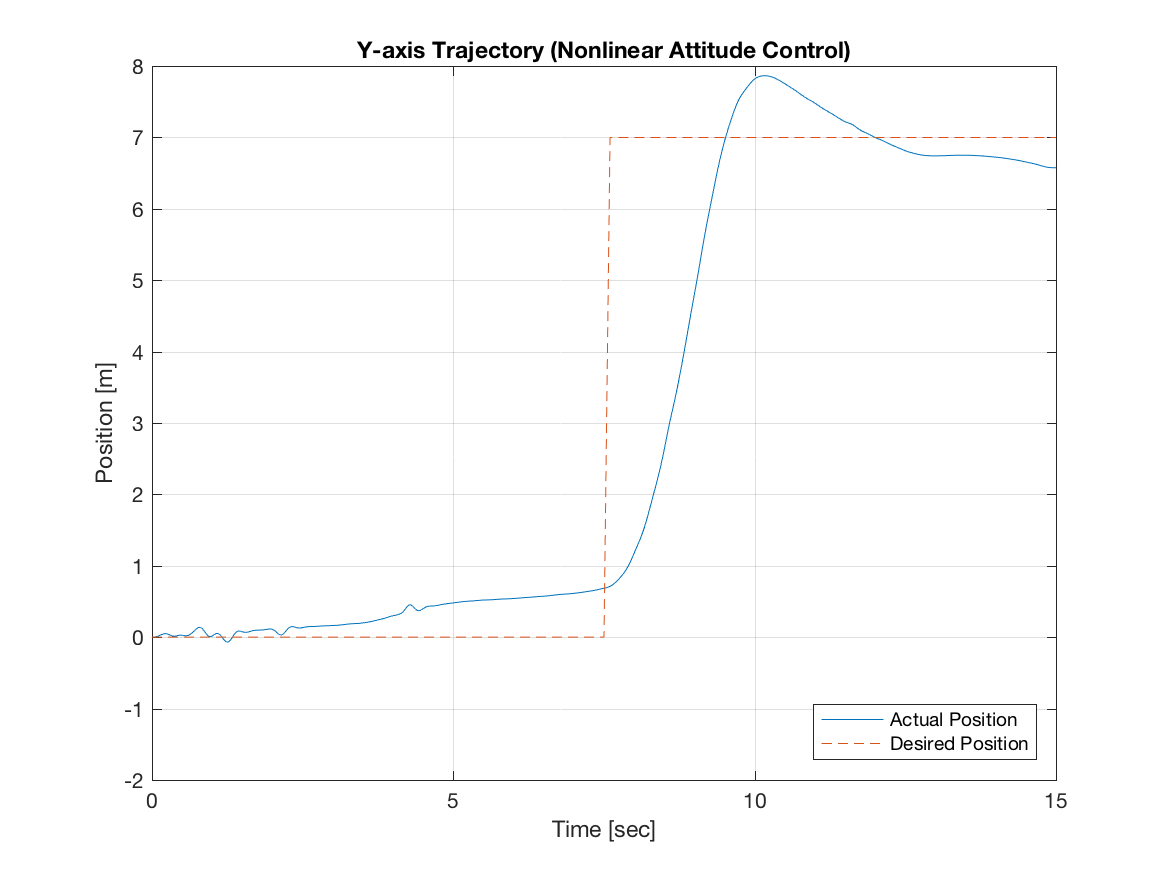
\includegraphics[width=0.45\textwidth]{graphics/experiment_plots/roll_plus_non_position_y.png}
    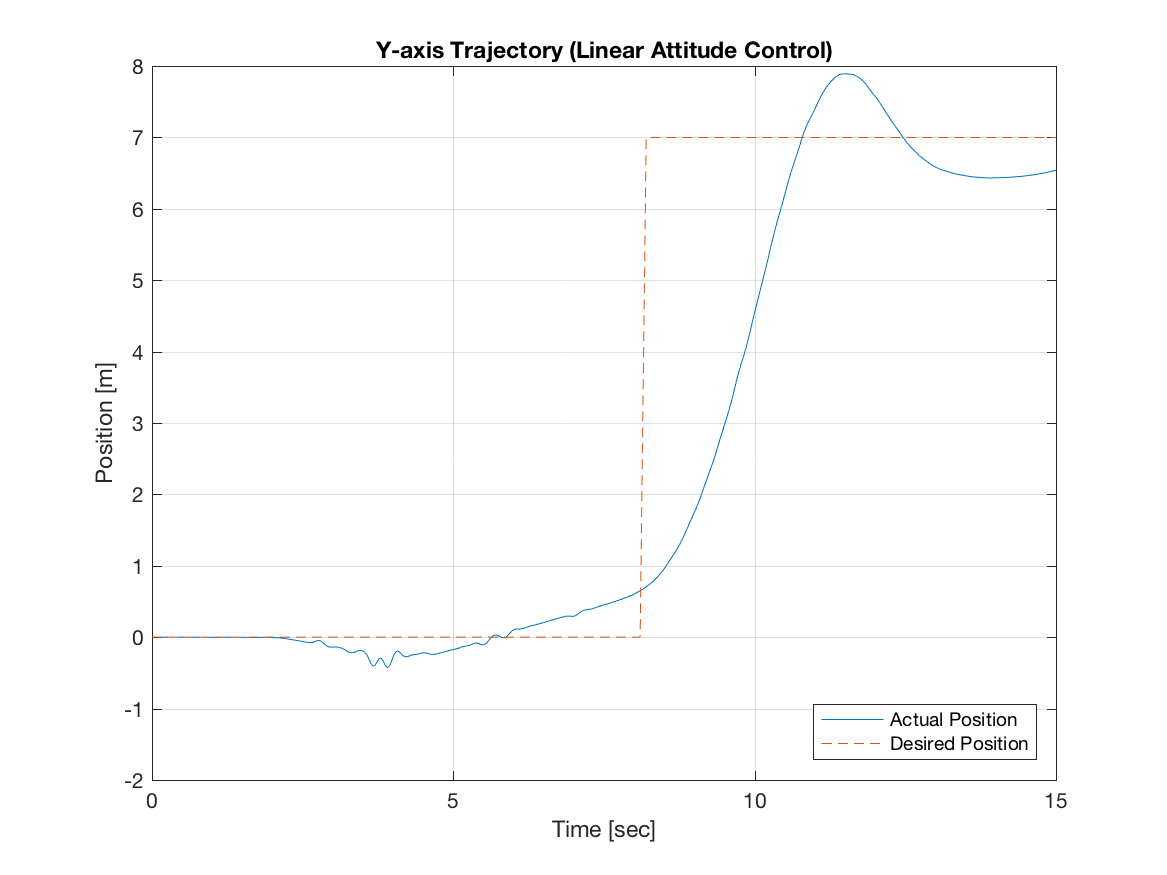
\includegraphics[width=0.45\textwidth]{graphics/experiment_plots/roll_plus_pid_position_y.png}
    
    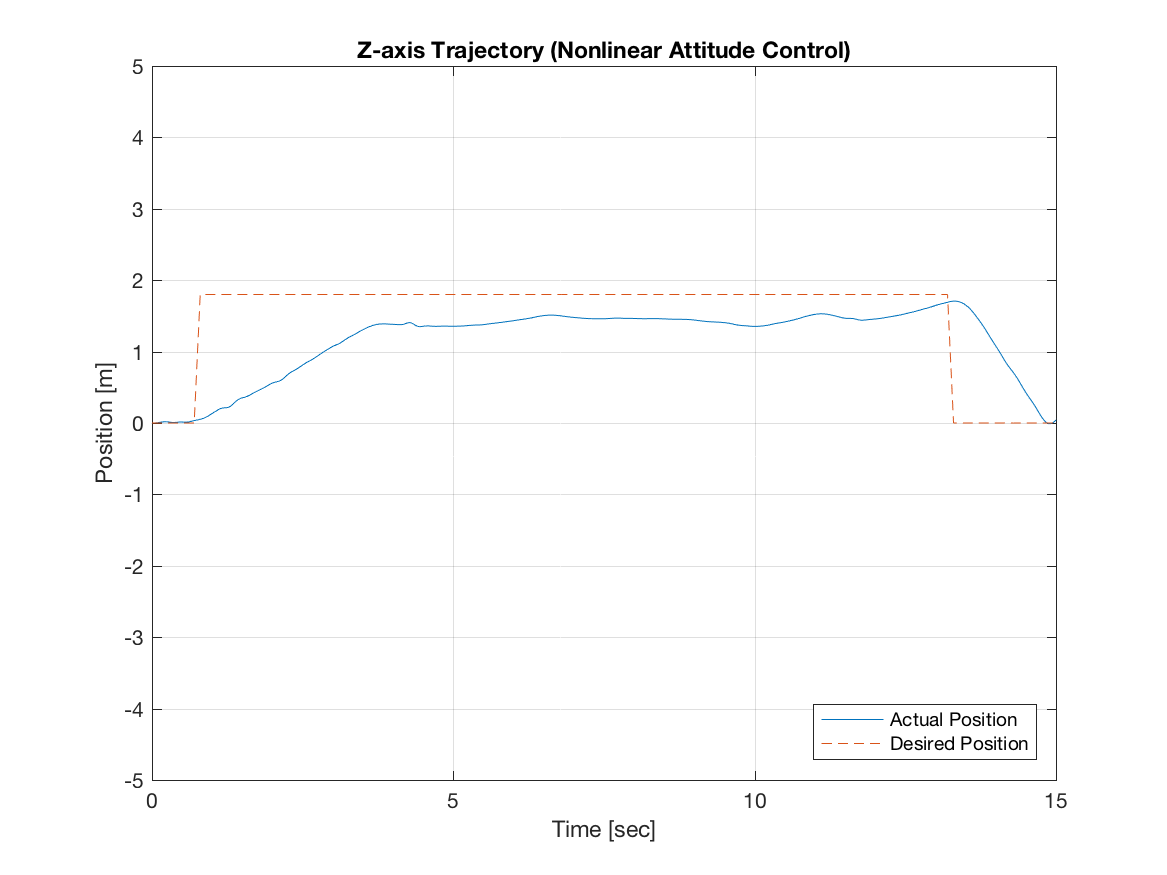
\includegraphics[width=0.45\textwidth]{graphics/experiment_plots/roll_plus_non_position_z.png}
    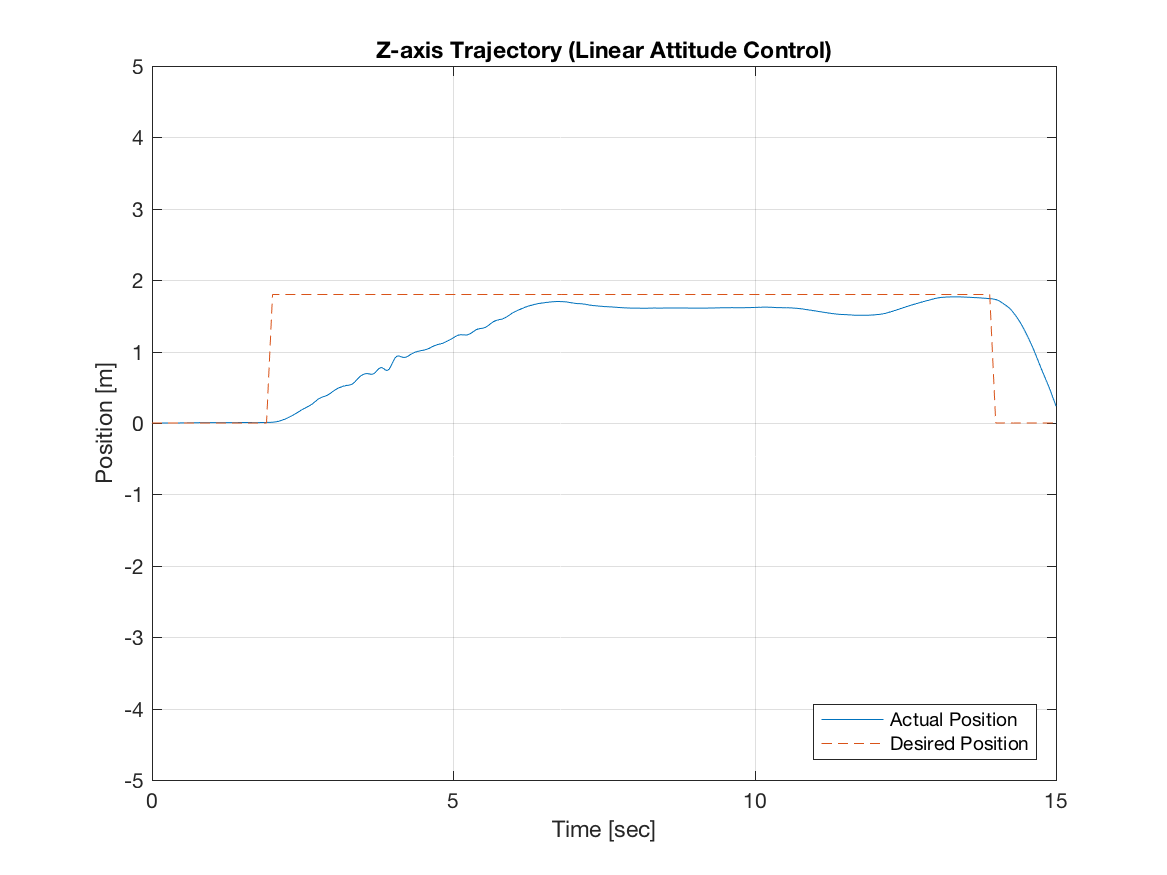
\includegraphics[width=0.45\textwidth]{graphics/experiment_plots/roll_plus_pid_position_z.png}

    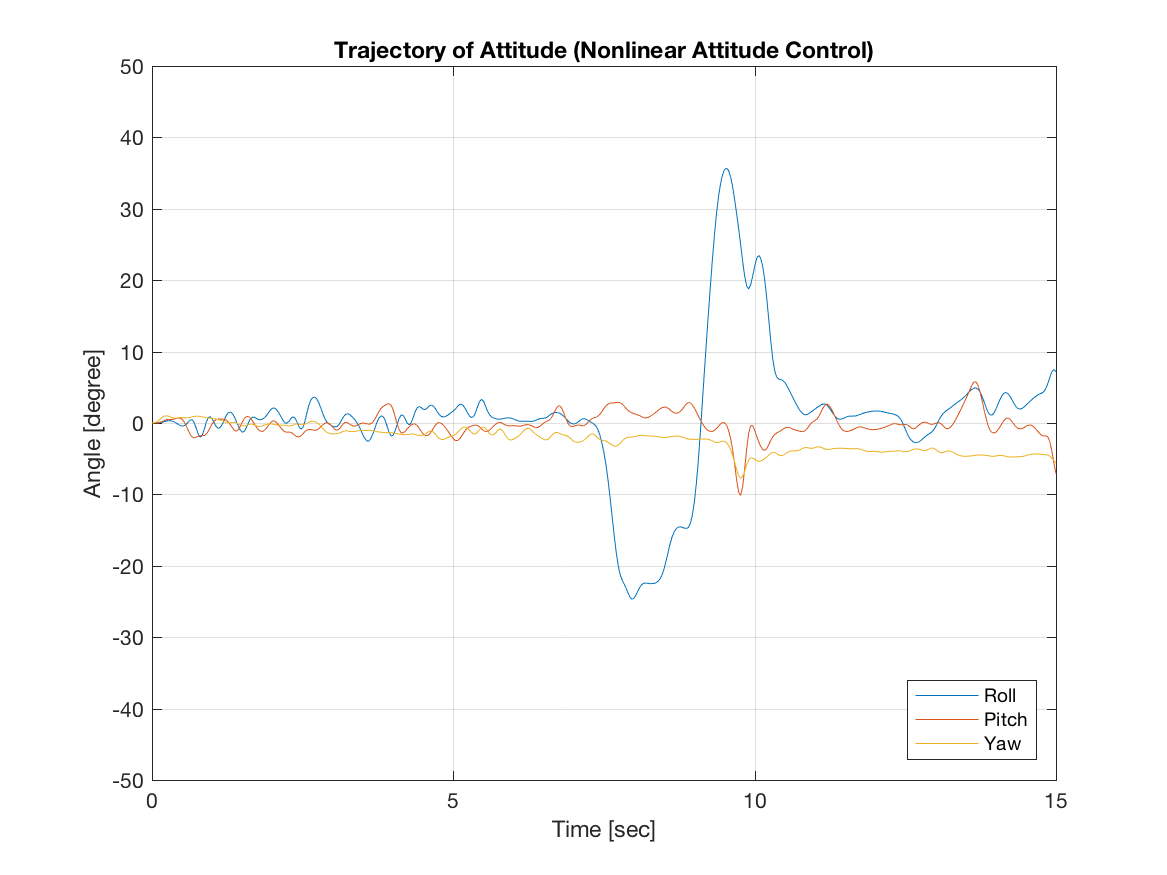
\includegraphics[width=0.45\textwidth]{graphics/experiment_plots/roll_plus_non_attitude.png}
    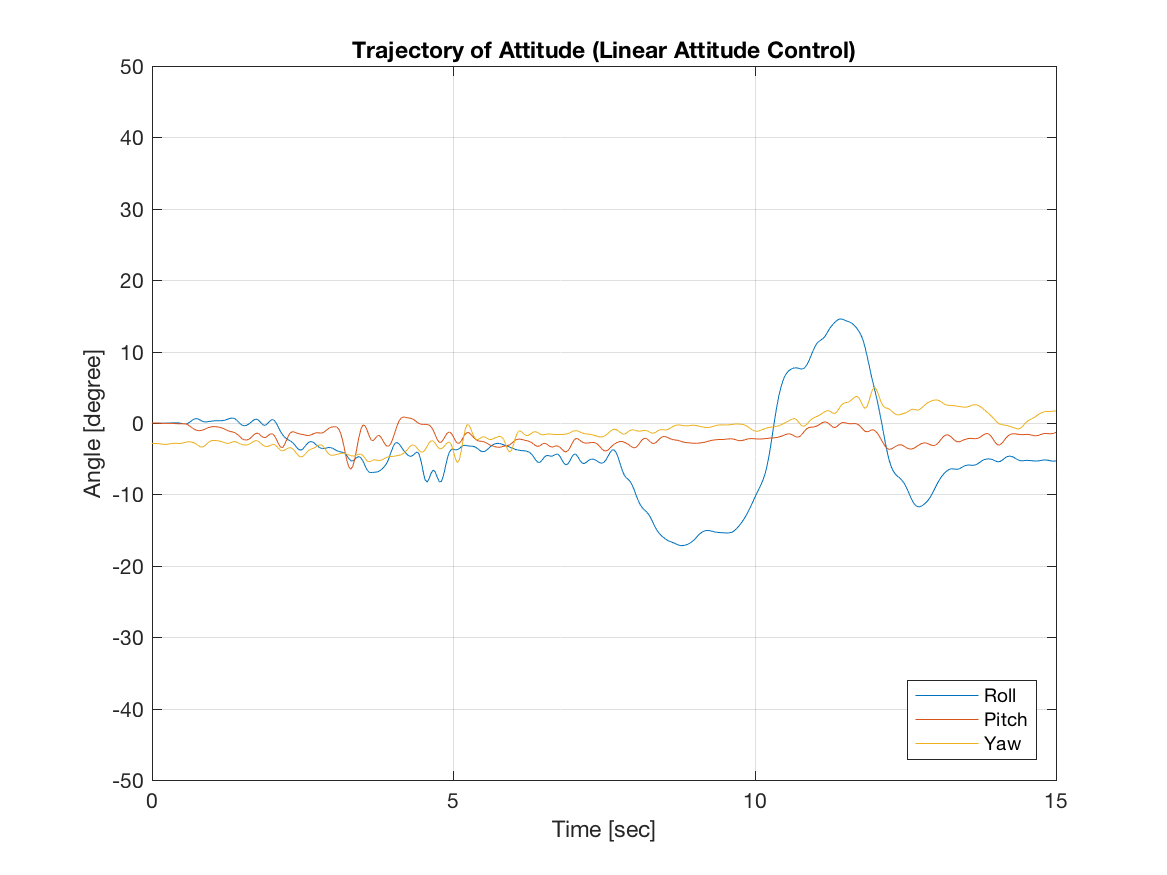
\includegraphics[width=0.45\textwidth]{graphics/experiment_plots/roll_plus_pid_attitude.png}
    \caption{Experiment Result (Case 2)}
    \label{fig:exp_roll_plus}
\end{figure}

\begin{figure}
    \centering
    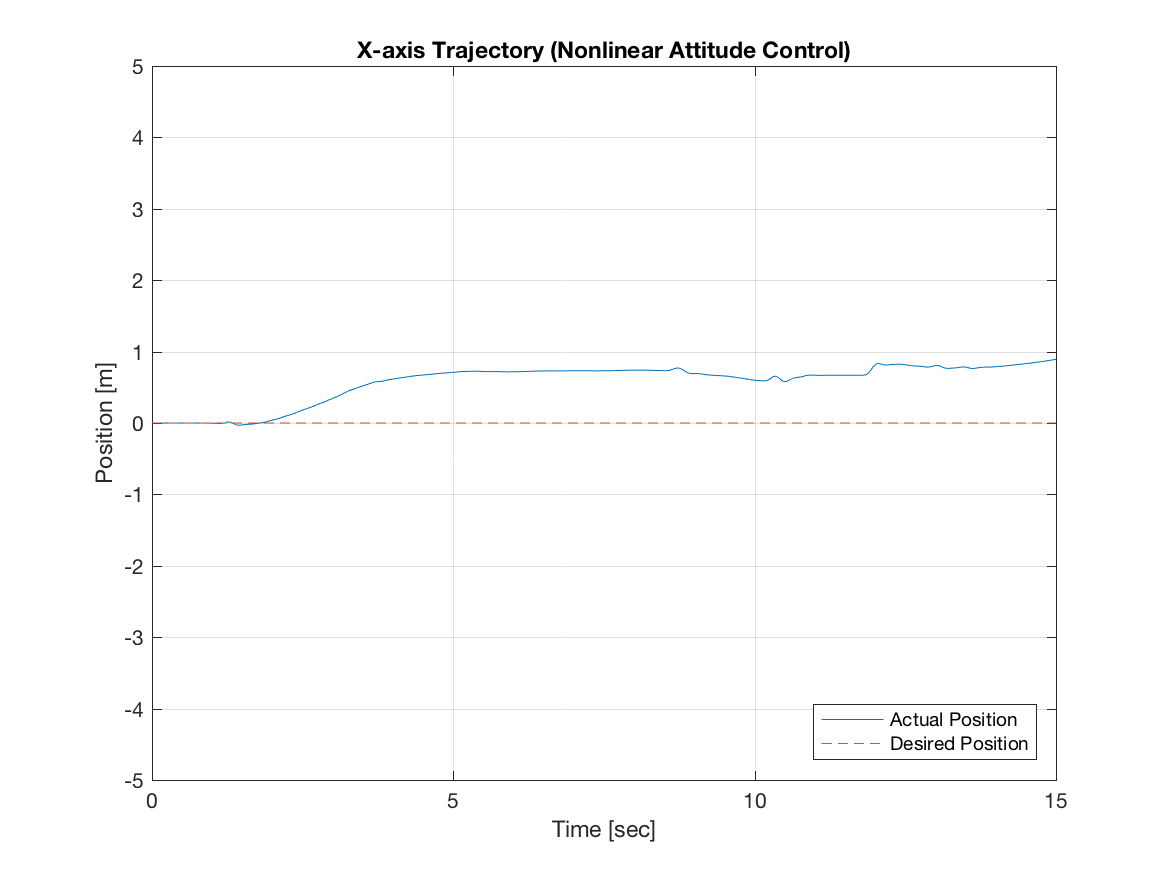
\includegraphics[width=0.45\textwidth]{graphics/experiment_plots/roll_minus_non_position_x.png}
    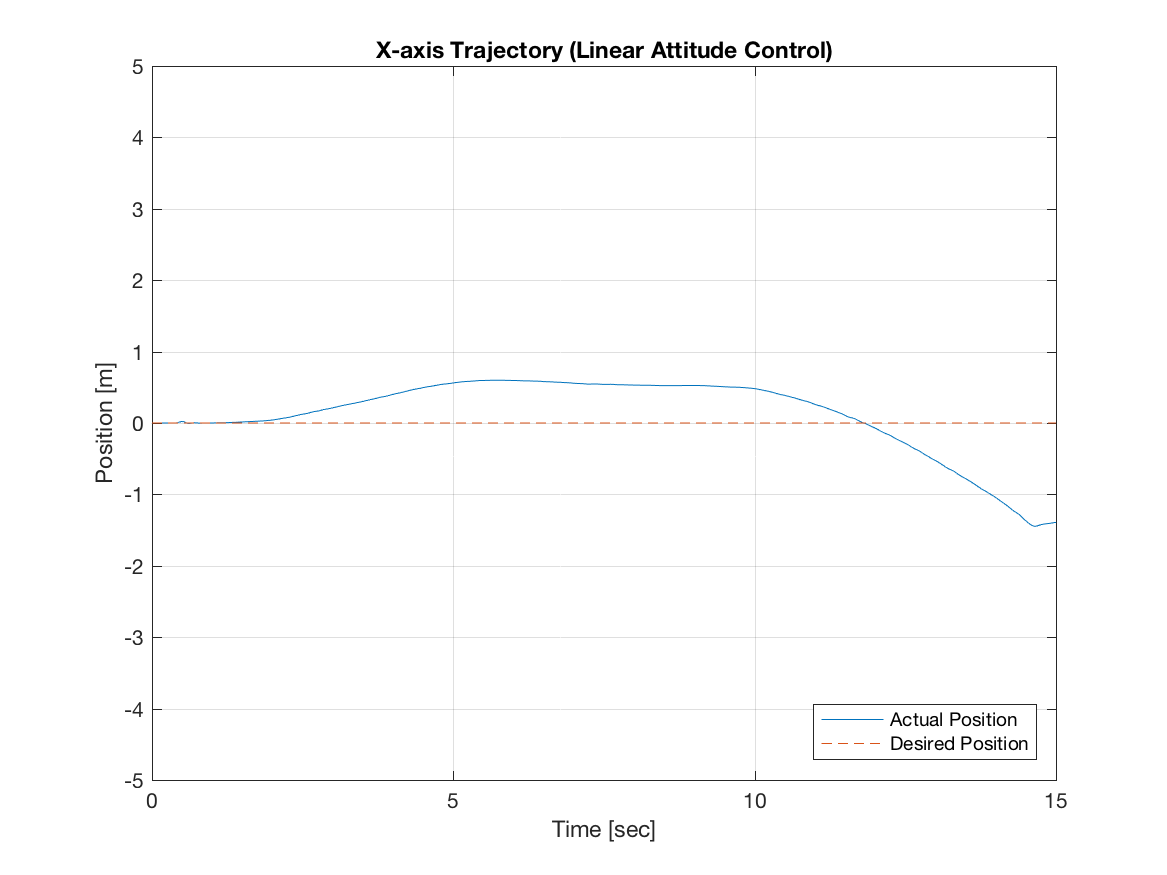
\includegraphics[width=0.45\textwidth]{graphics/experiment_plots/roll_minus_pid_position_x.png}
    
    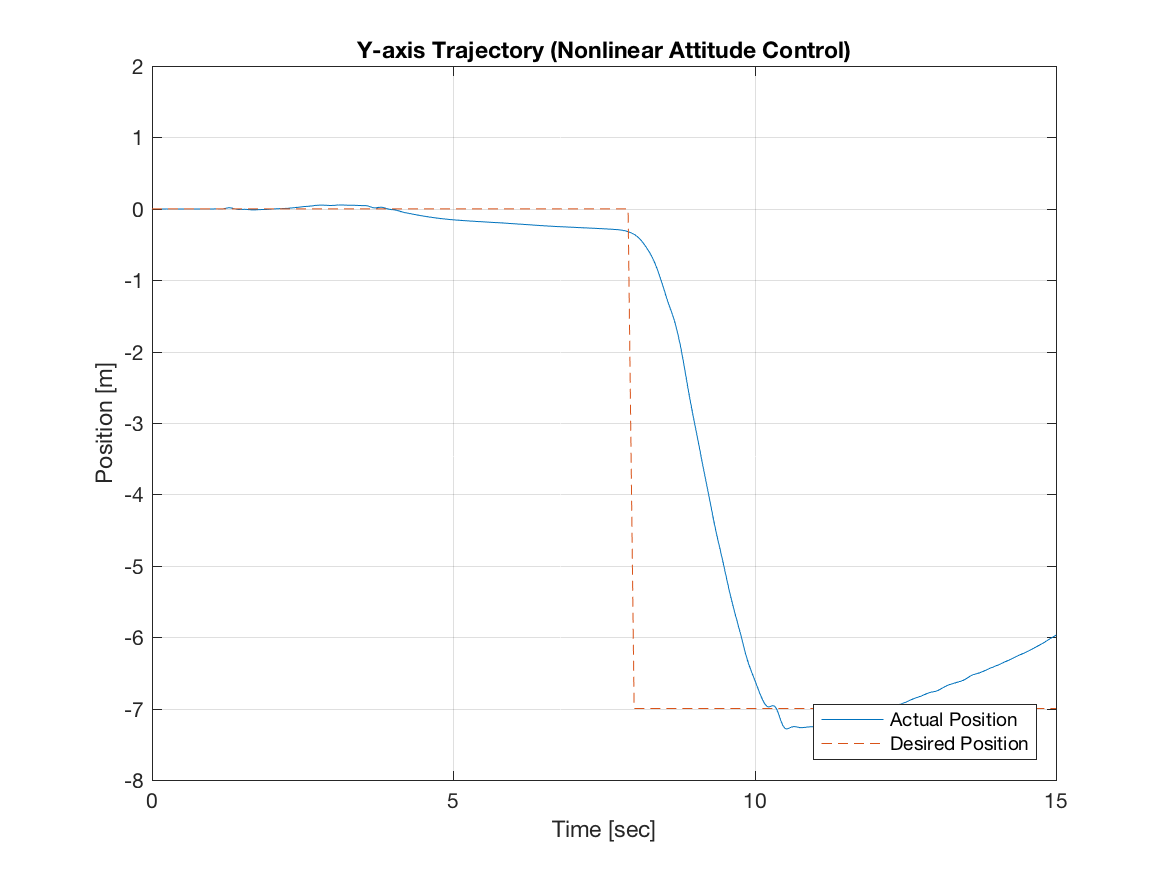
\includegraphics[width=0.45\textwidth]{graphics/experiment_plots/roll_minus_non_position_y.png}
    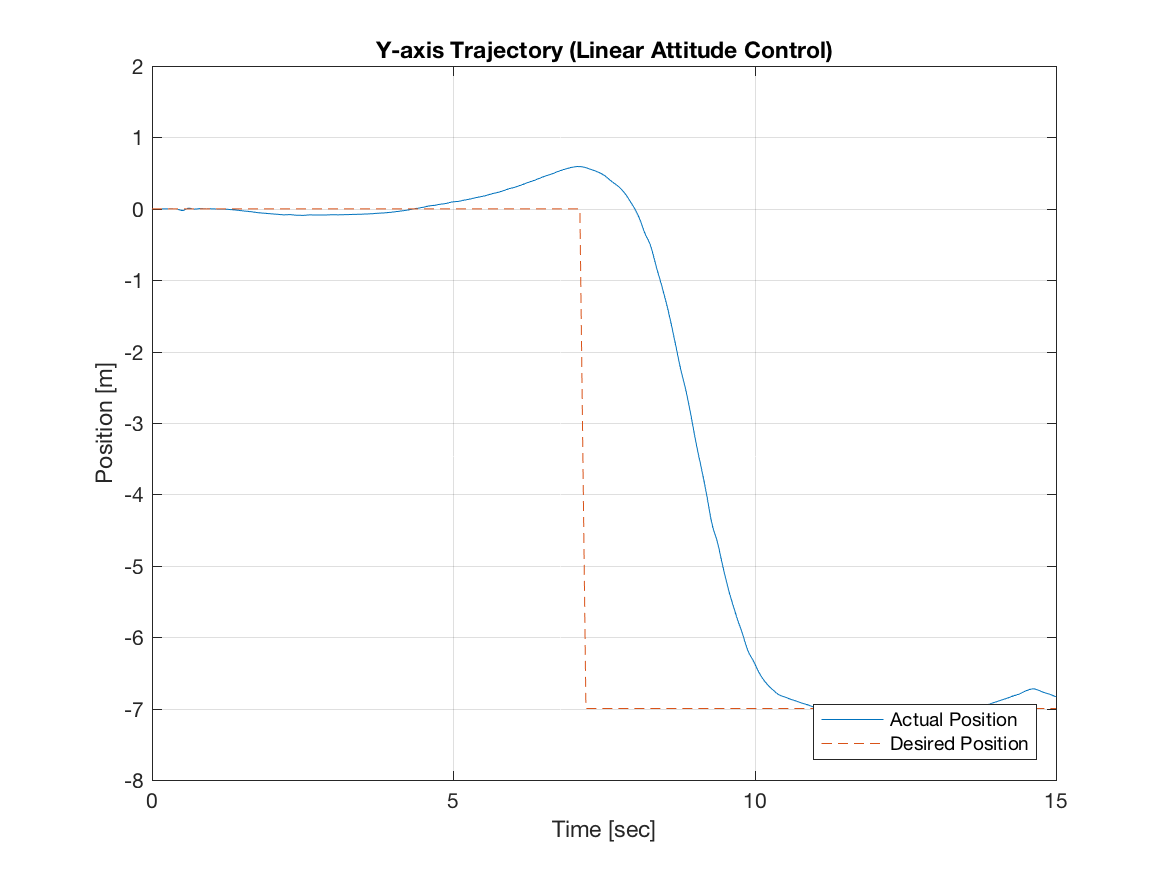
\includegraphics[width=0.45\textwidth]{graphics/experiment_plots/roll_minus_pid_position_y.png}
    
    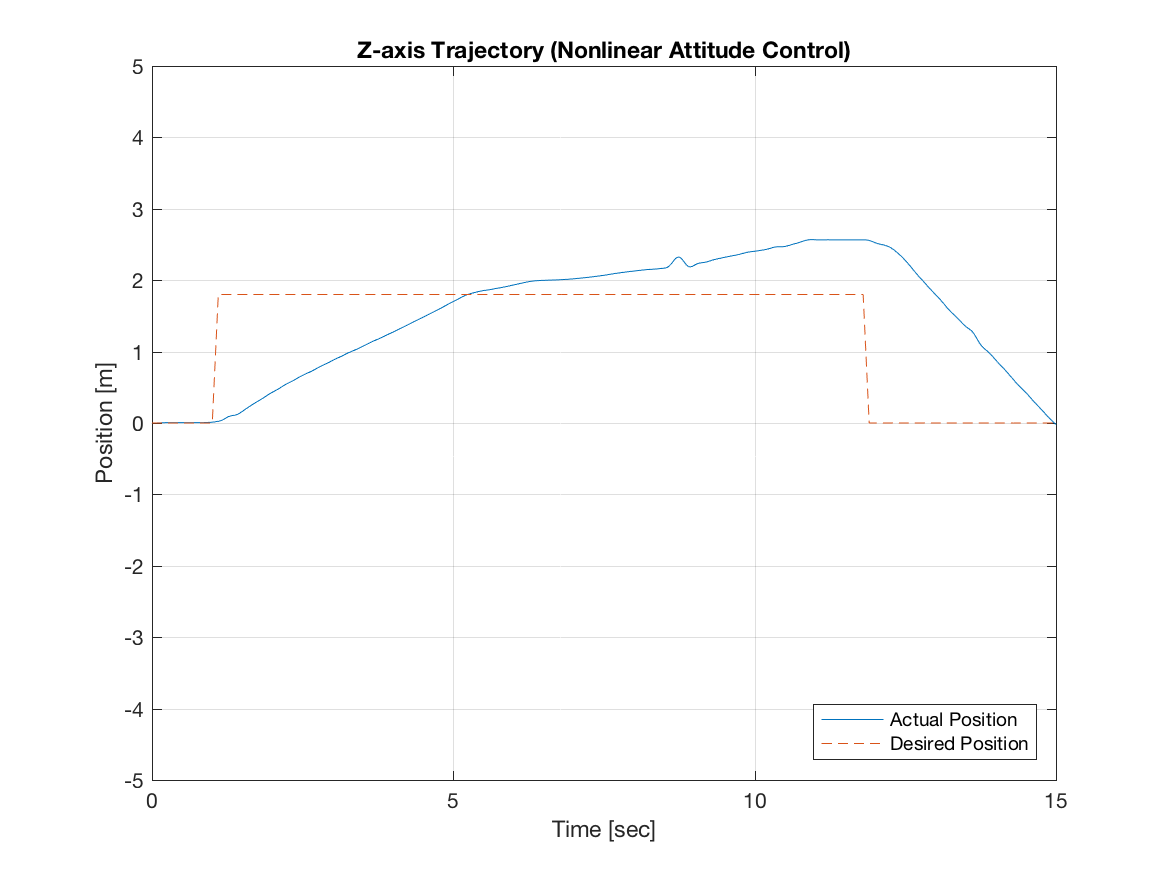
\includegraphics[width=0.45\textwidth]{graphics/experiment_plots/roll_minus_non_position_z.png}
    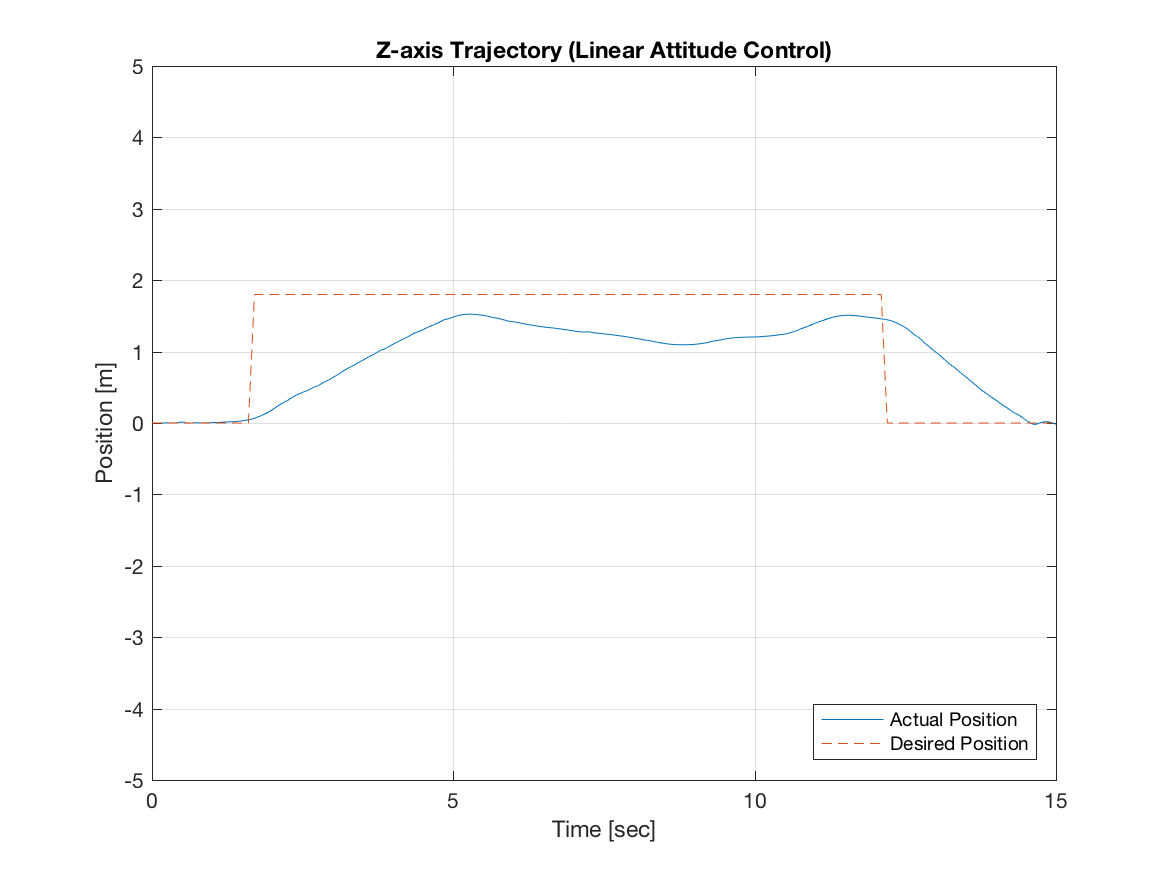
\includegraphics[width=0.45\textwidth]{graphics/experiment_plots/roll_minus_pid_position_z.png}

    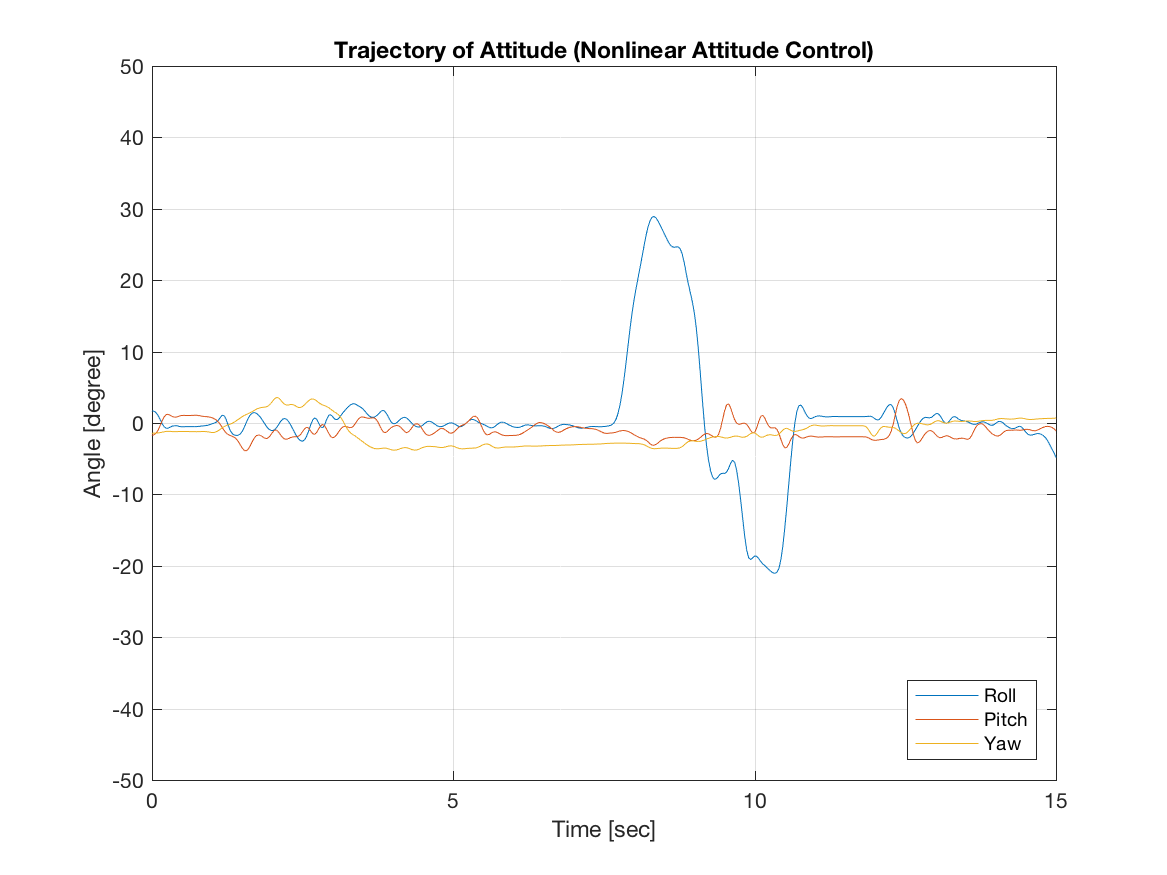
\includegraphics[width=0.45\textwidth]{graphics/experiment_plots/roll_minus_non_attitude.png}
    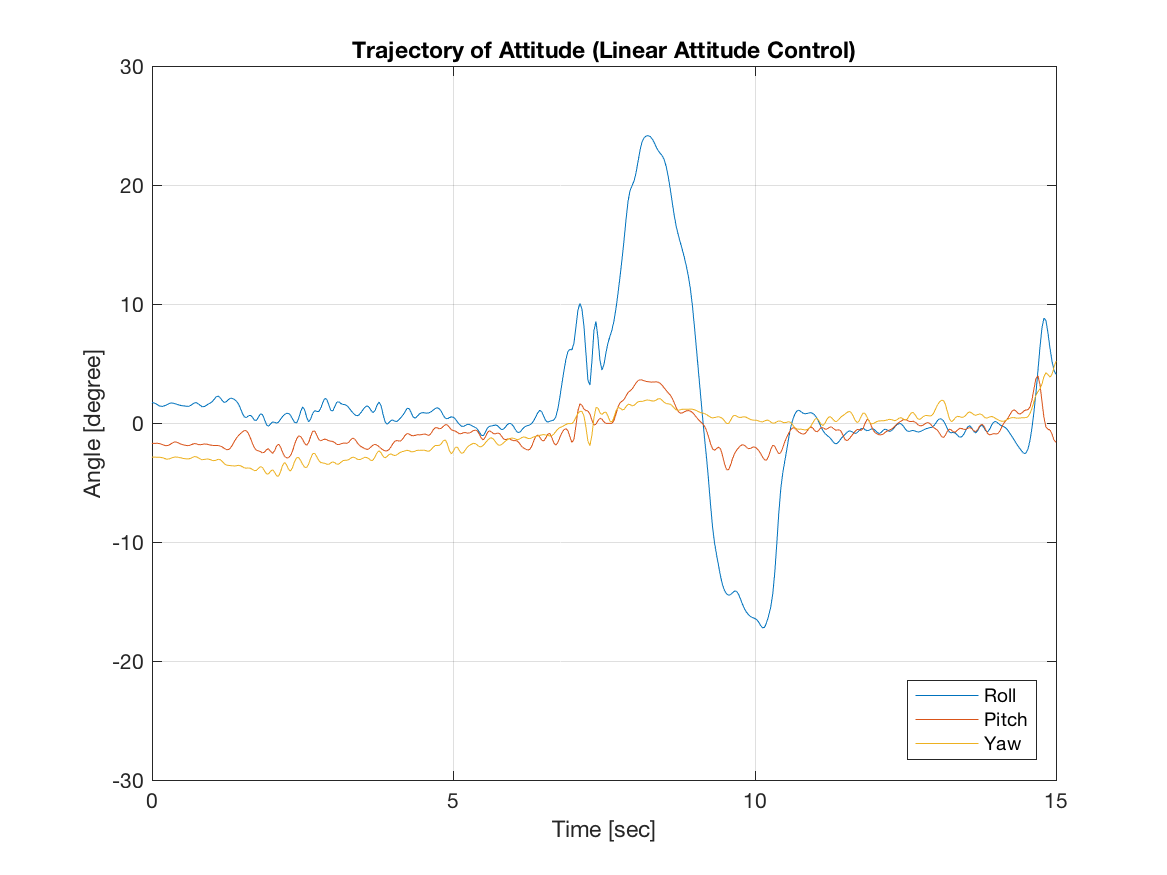
\includegraphics[width=0.45\textwidth]{graphics/experiment_plots/roll_minus_pid_attitude.png}
    \caption{Experiment Result (Case 3)}
    \label{fig:exp_roll_minus}
\end{figure}

\begin{figure}
    \centering
    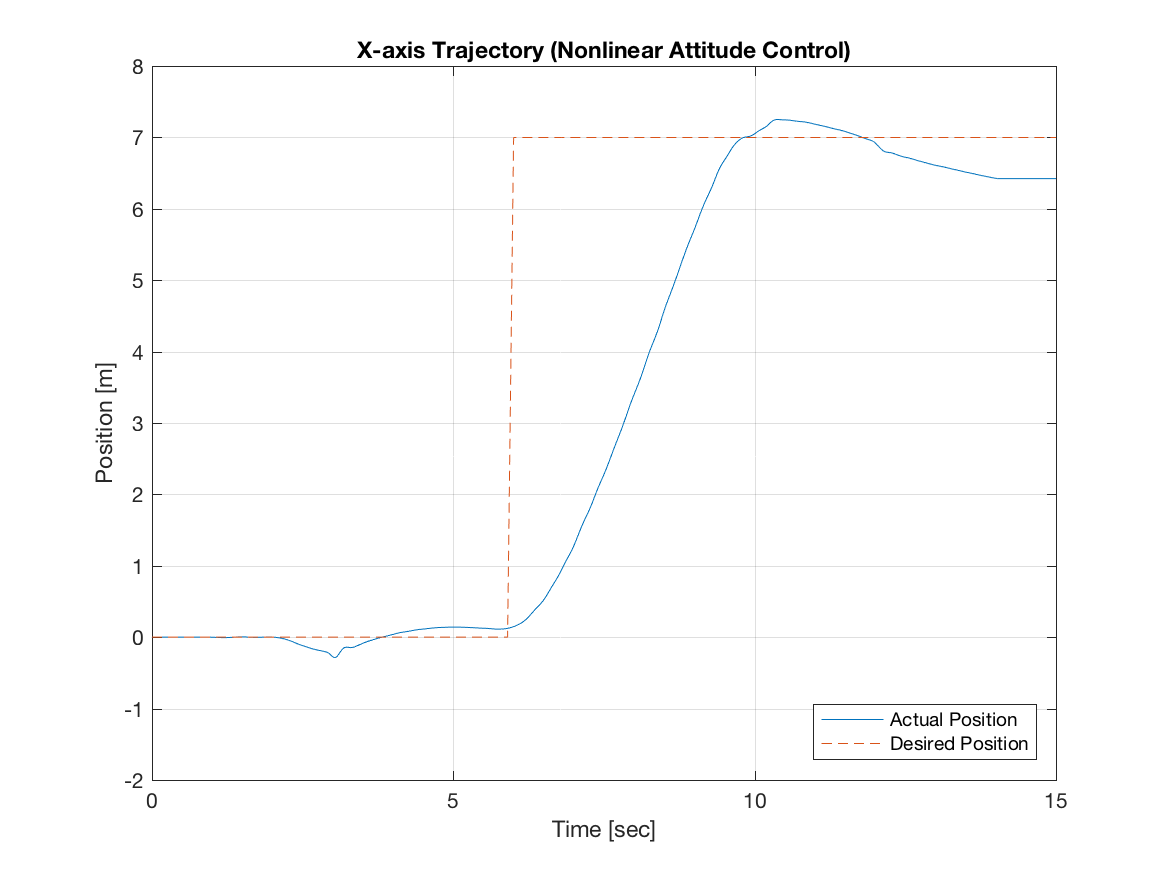
\includegraphics[width=0.45\textwidth]{graphics/experiment_plots/pitch_plus_non_position_x.png}
    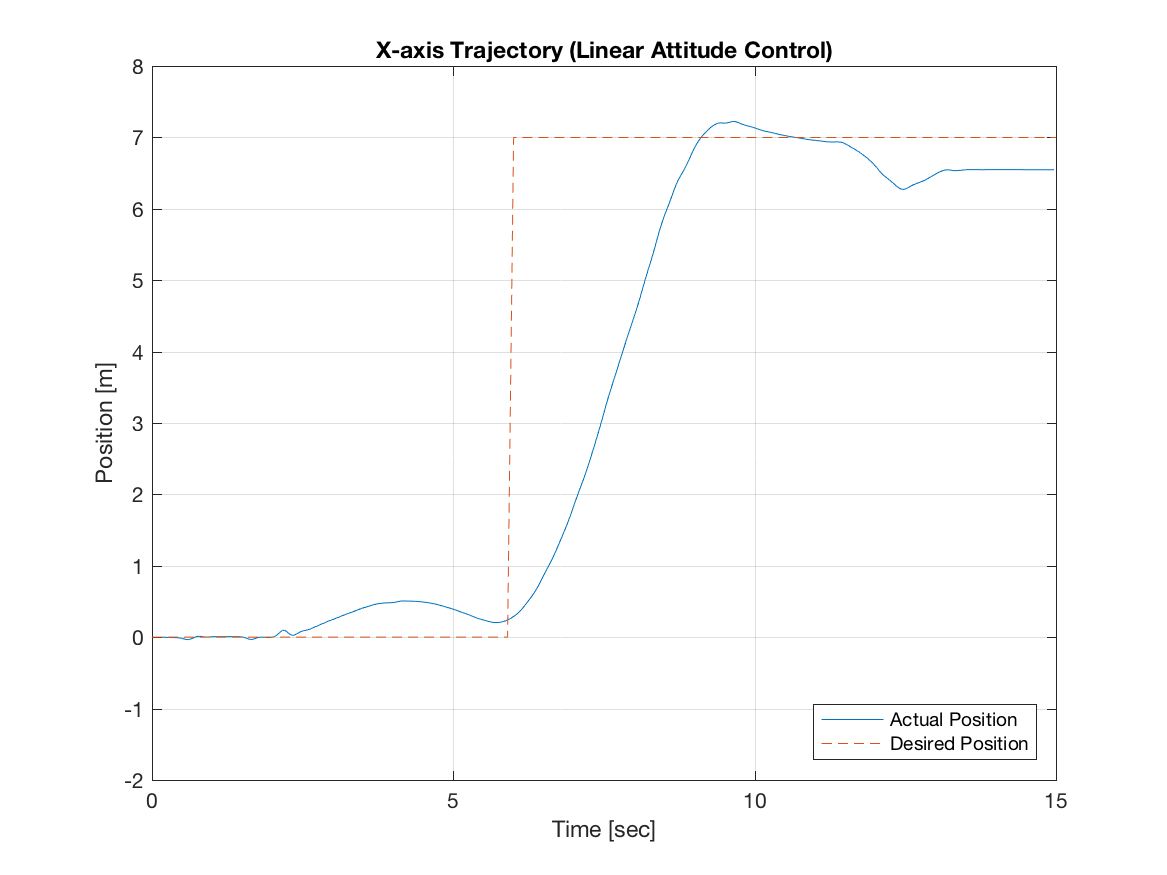
\includegraphics[width=0.45\textwidth]{graphics/experiment_plots/pitch_plus_pid_position_x.png}
    
    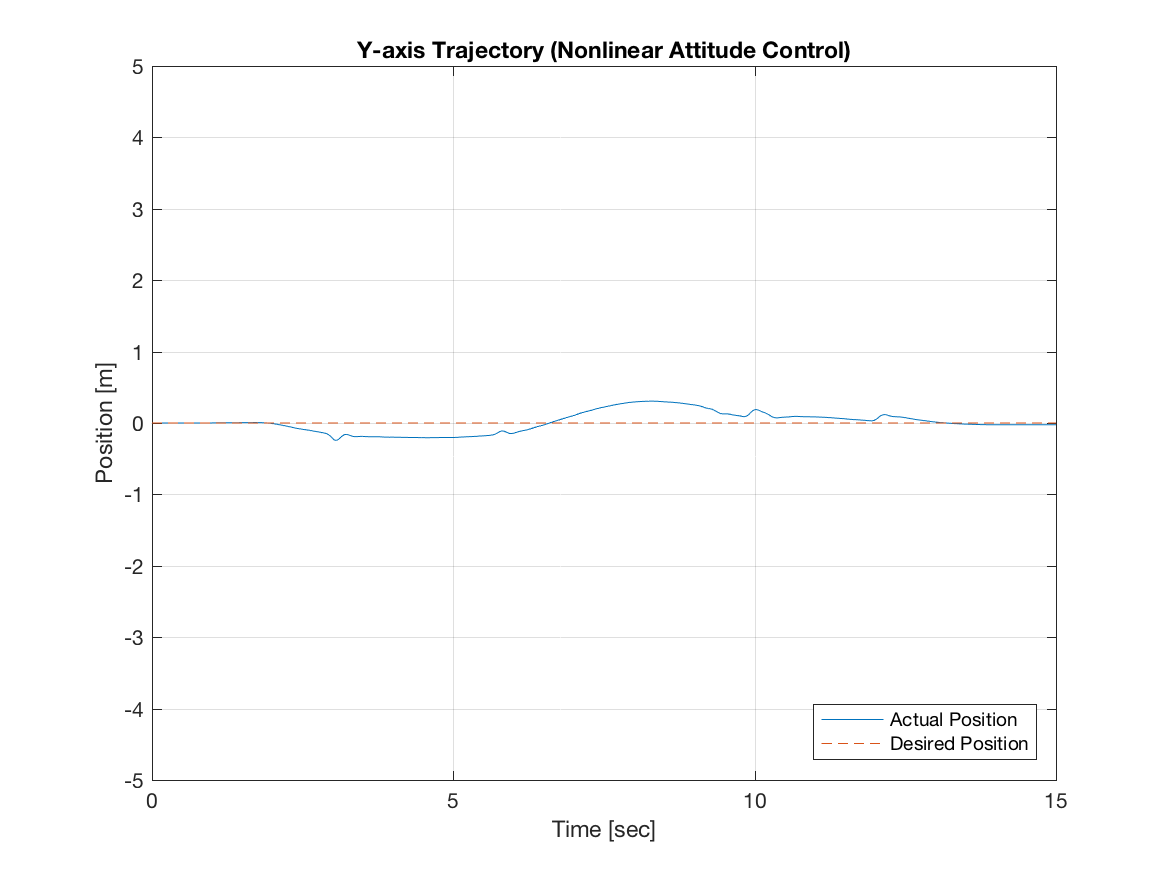
\includegraphics[width=0.45\textwidth]{graphics/experiment_plots/pitch_plus_non_position_y.png}
    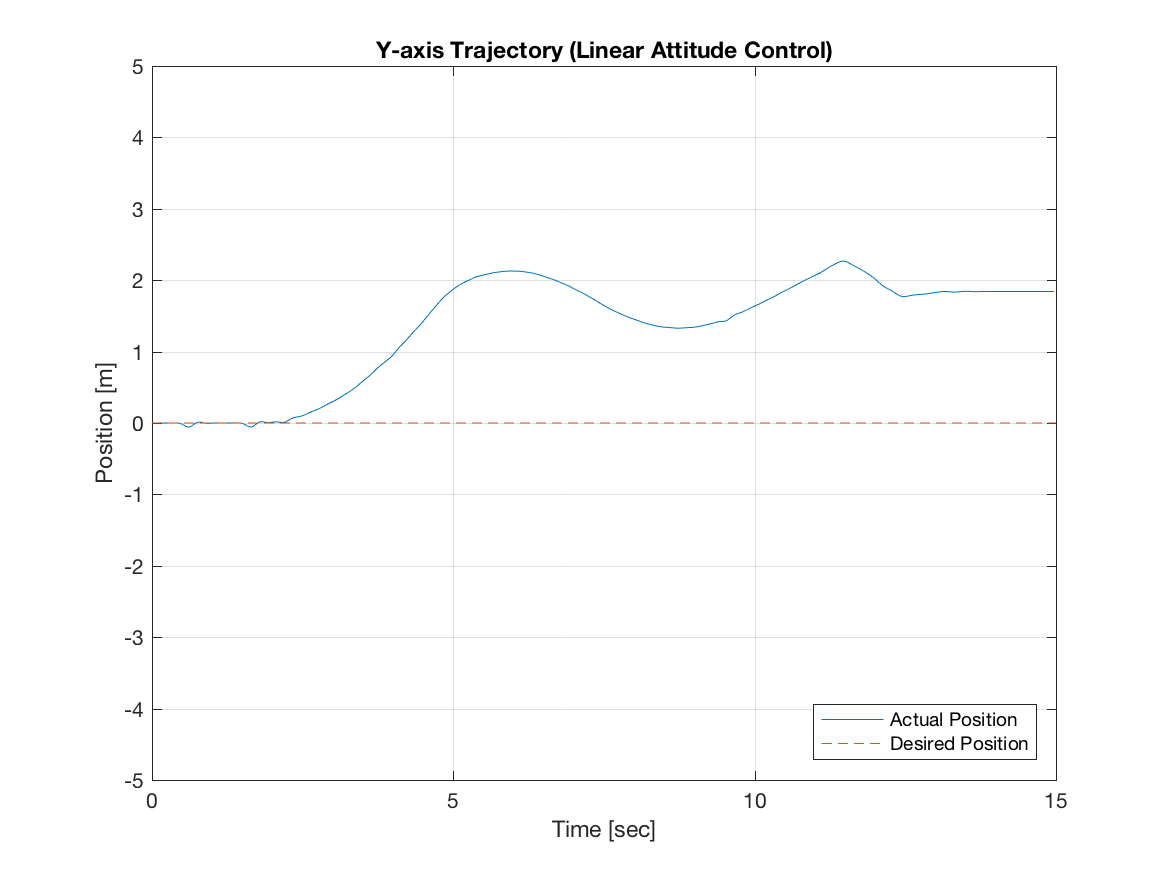
\includegraphics[width=0.45\textwidth]{graphics/experiment_plots/pitch_plus_pid_position_y.png}
    
    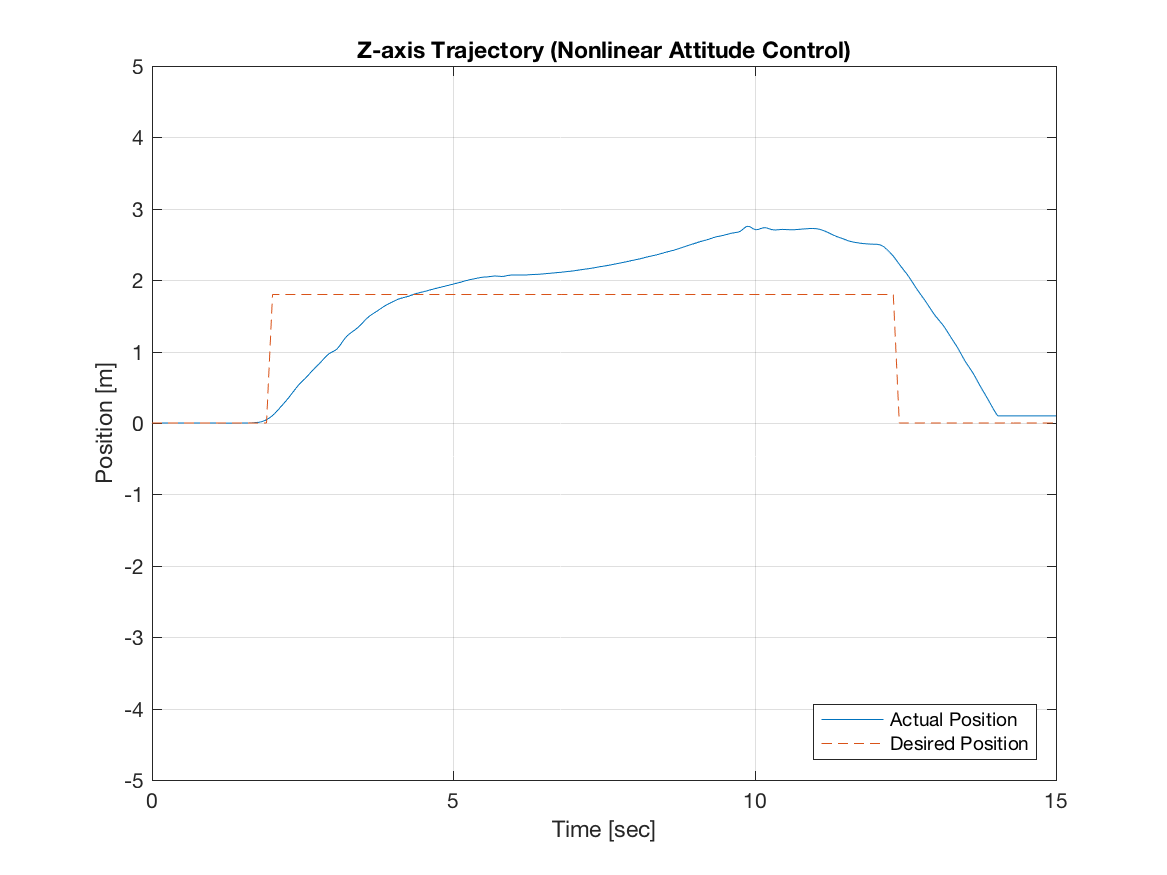
\includegraphics[width=0.45\textwidth]{graphics/experiment_plots/pitch_plus_non_position_z.png}
    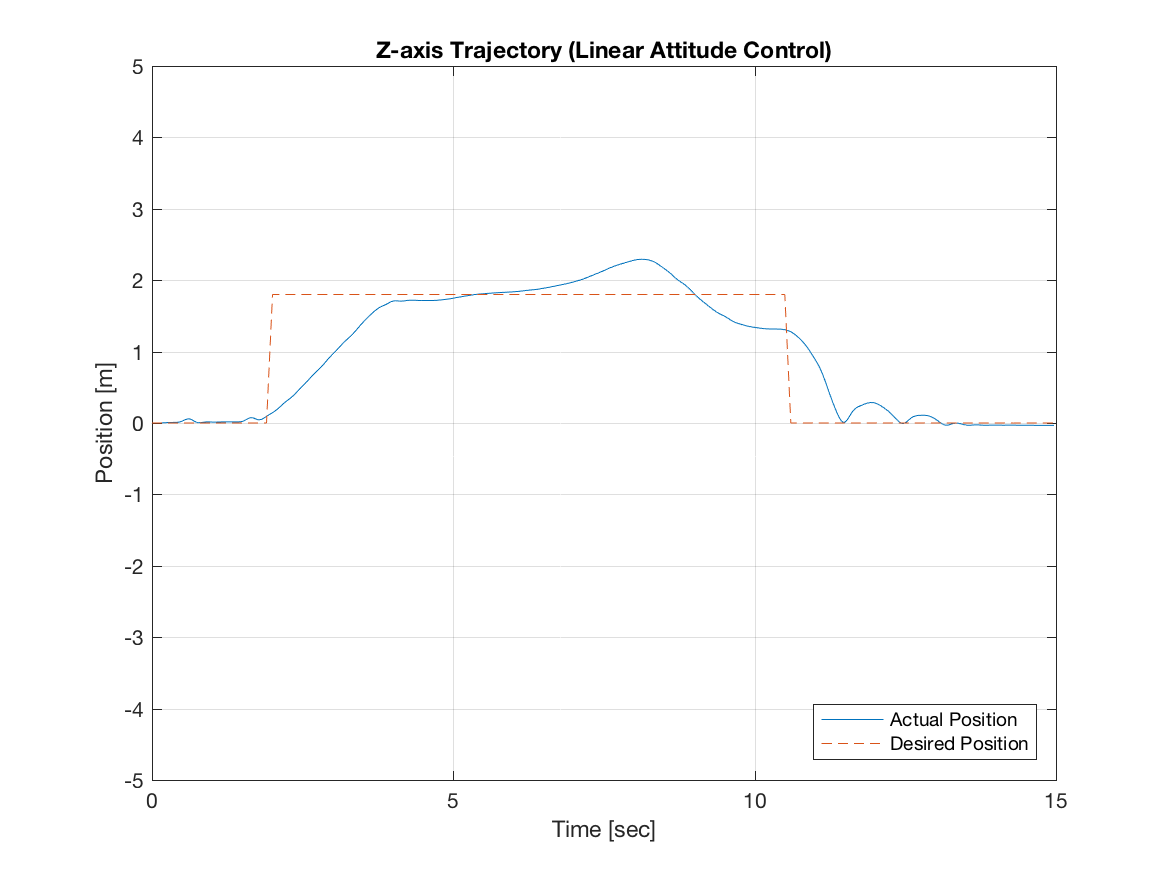
\includegraphics[width=0.45\textwidth]{graphics/experiment_plots/pitch_plus_pid_position_z.png}

    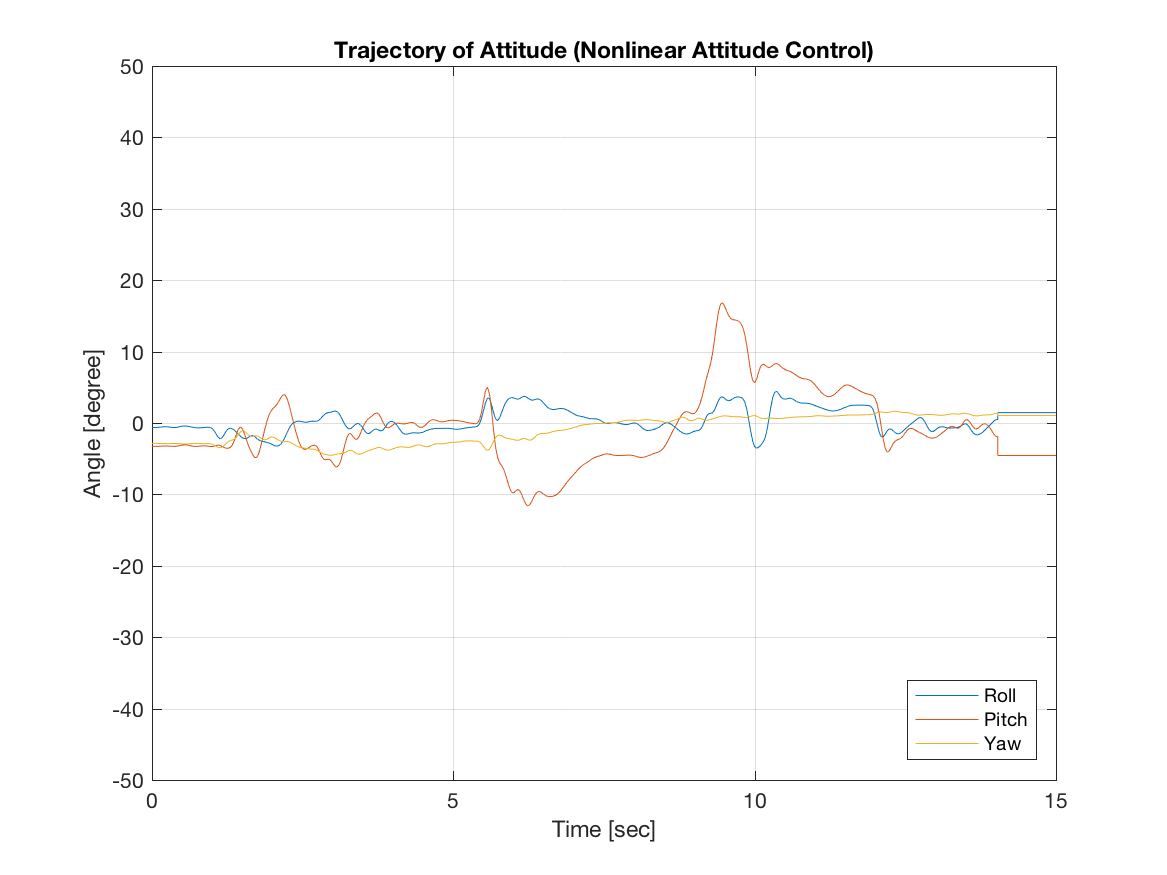
\includegraphics[width=0.45\textwidth]{graphics/experiment_plots/pitch_plus_non_attitude.png}
    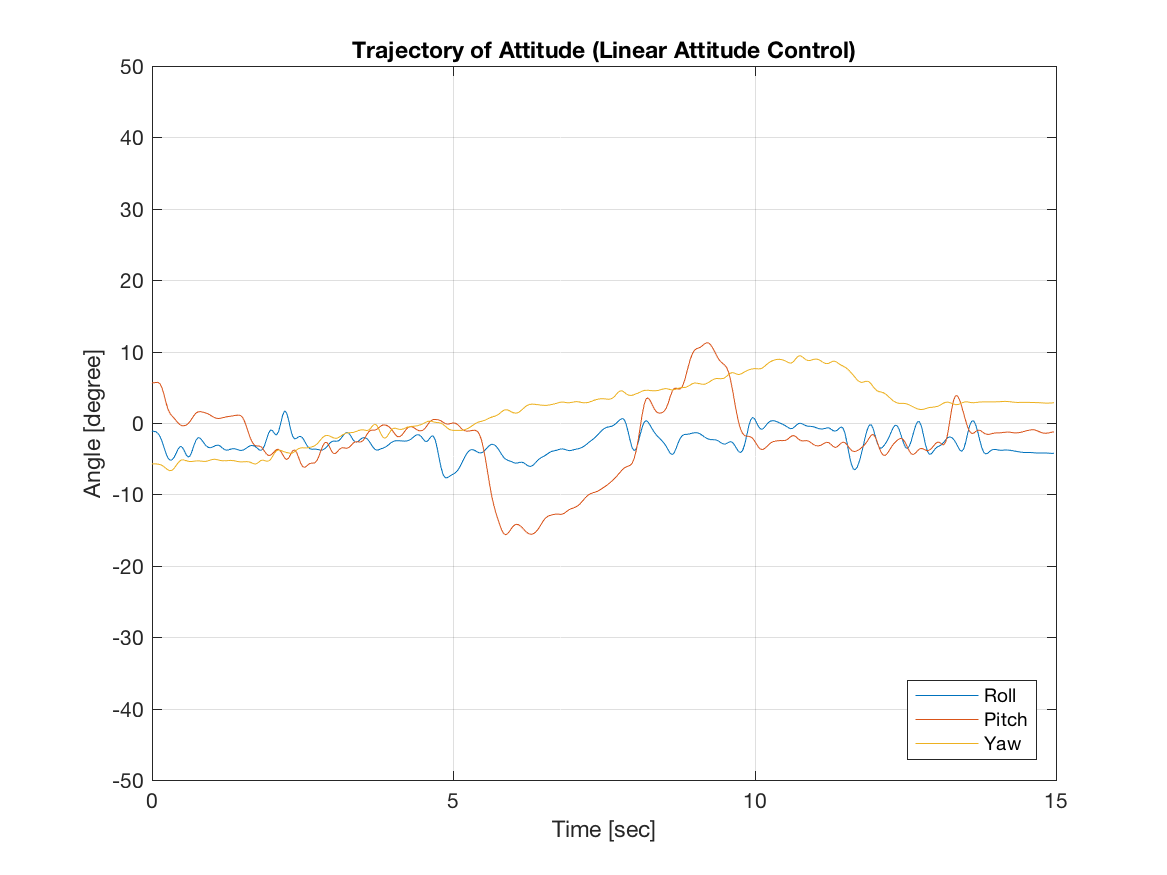
\includegraphics[width=0.45\textwidth]{graphics/experiment_plots/pitch_plus_pid_attitude.png}
    \caption{Experiment Result (Case 4)}
    \label{fig:exp_pitch_plus}
\end{figure}

\begin{figure}
    \centering
    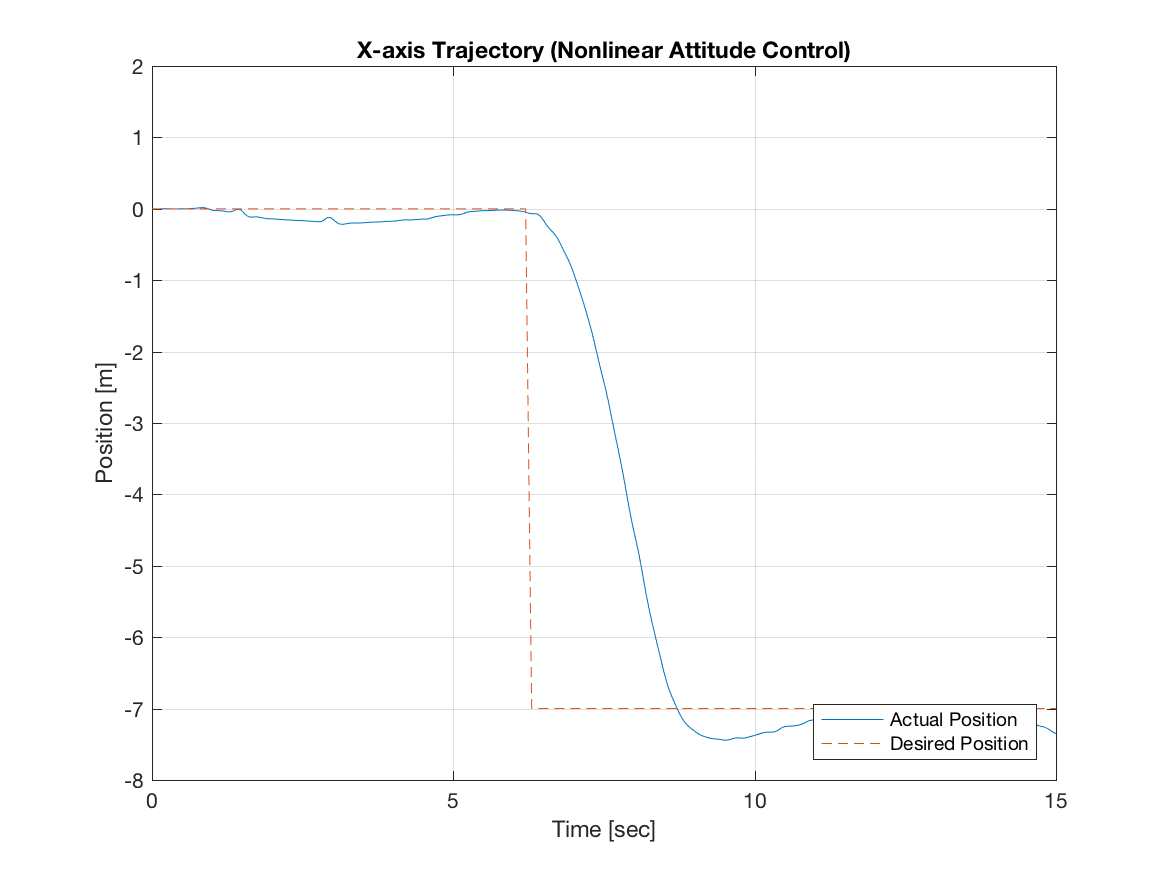
\includegraphics[width=0.45\textwidth]{graphics/experiment_plots/pitch_minus_non_position_x.png}
    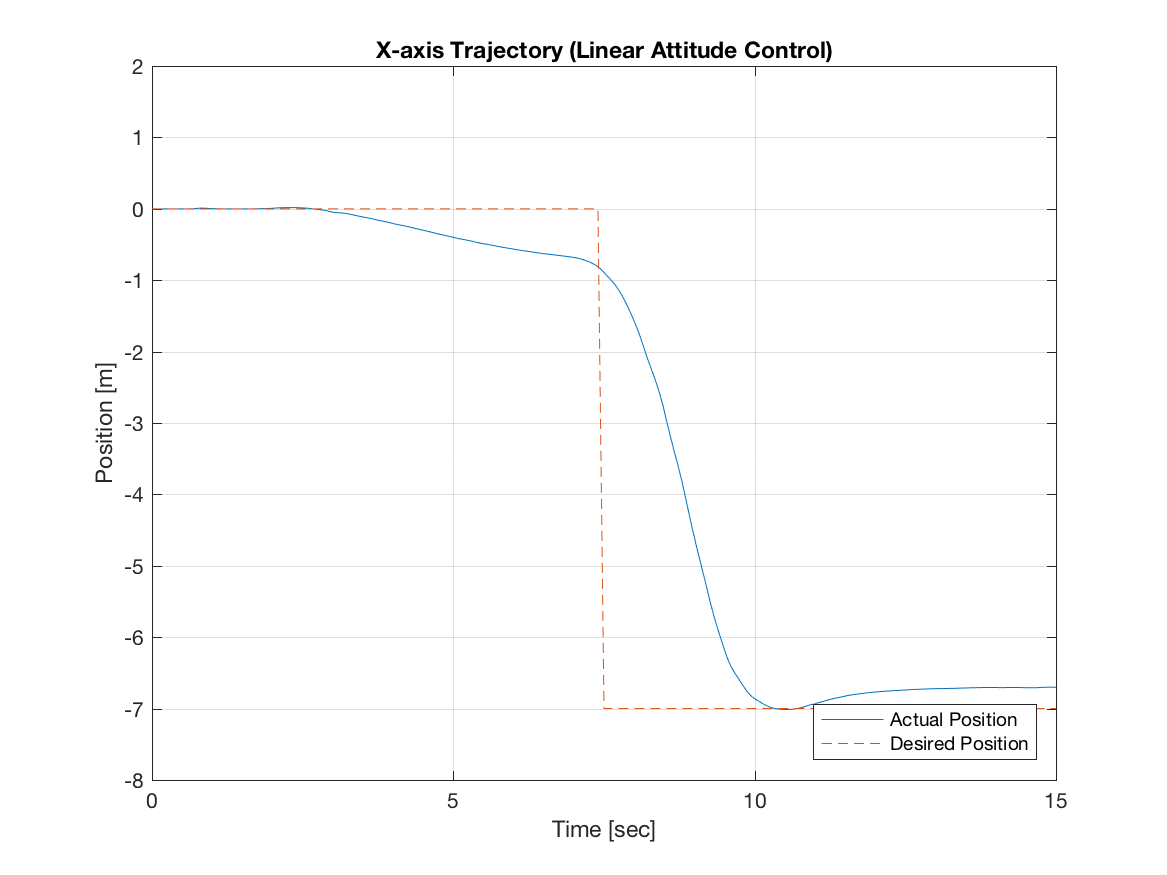
\includegraphics[width=0.45\textwidth]{graphics/experiment_plots/pitch_minus_pid_position_x.png}
    
    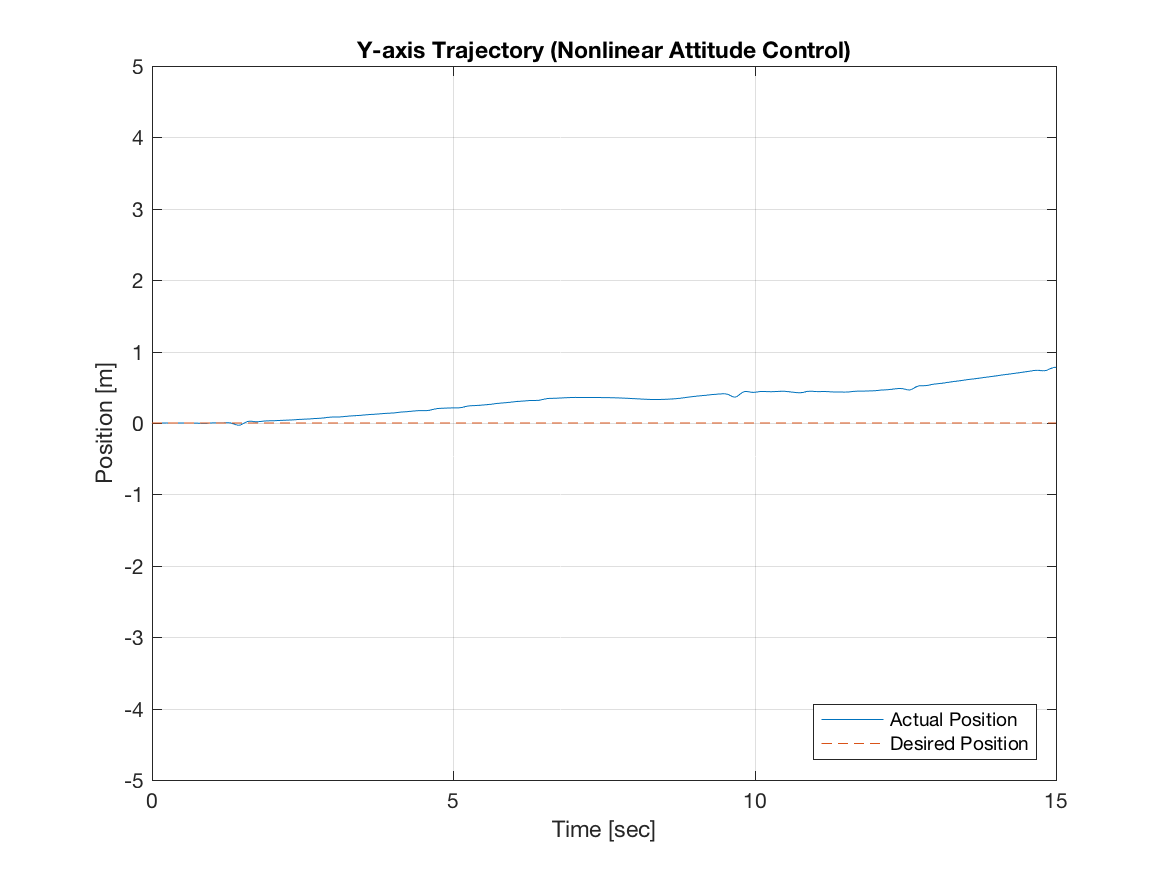
\includegraphics[width=0.45\textwidth]{graphics/experiment_plots/pitch_minus_non_position_y.png}
    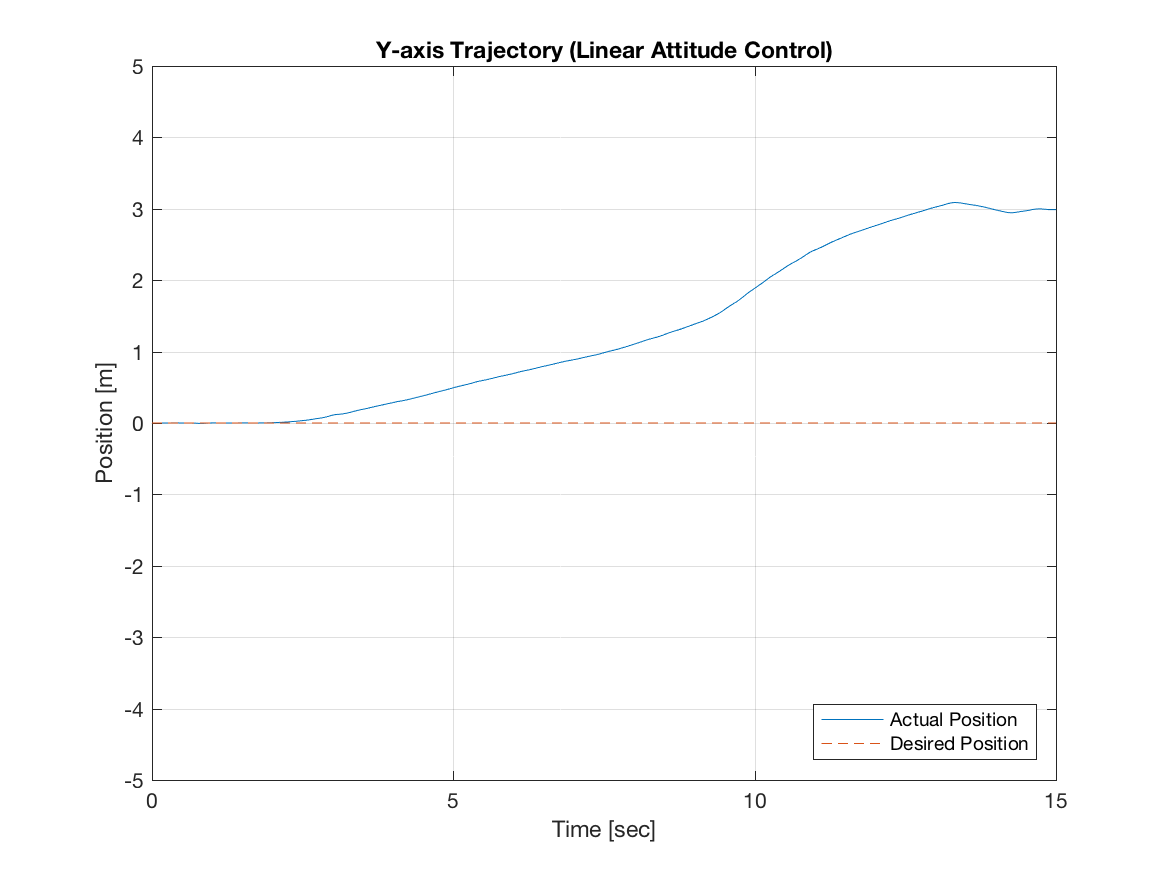
\includegraphics[width=0.45\textwidth]{graphics/experiment_plots/pitch_minus_pid_position_y.png}
    
    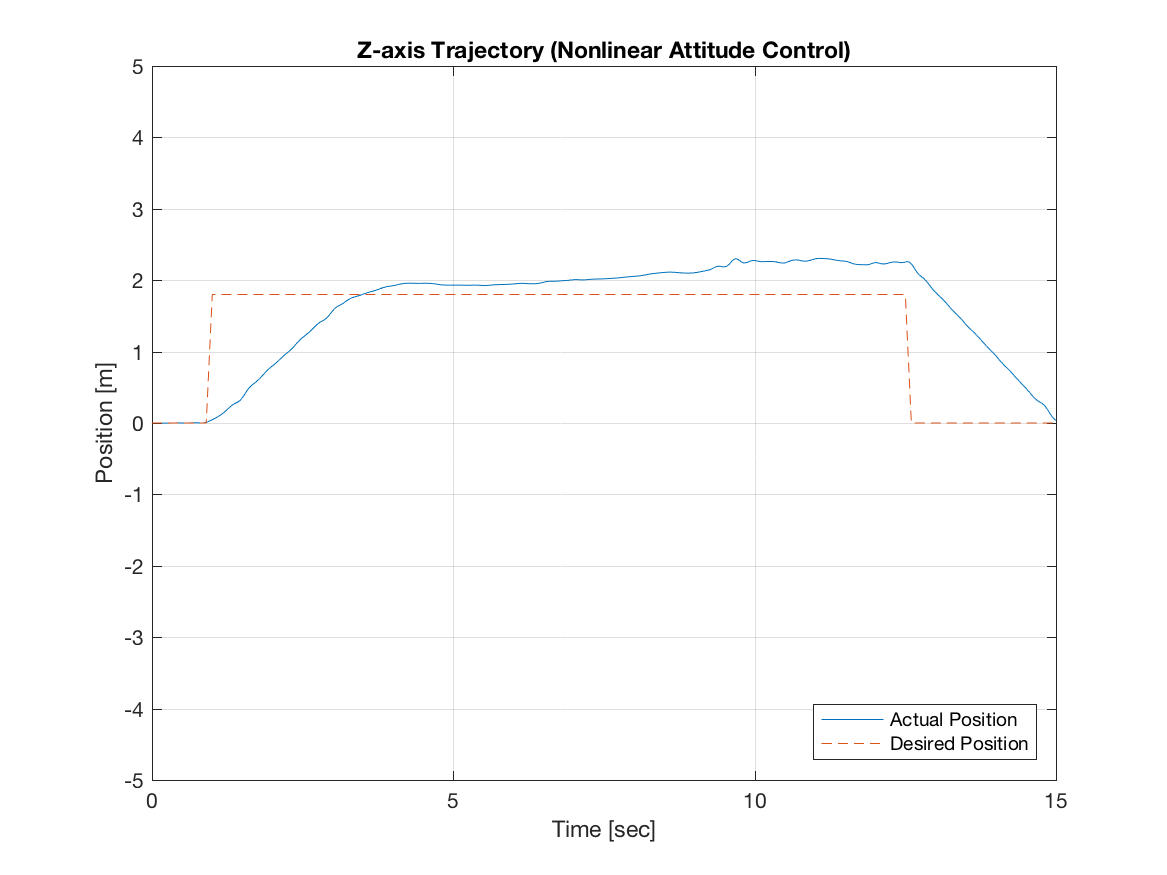
\includegraphics[width=0.45\textwidth]{graphics/experiment_plots/pitch_minus_non_position_z.png}
    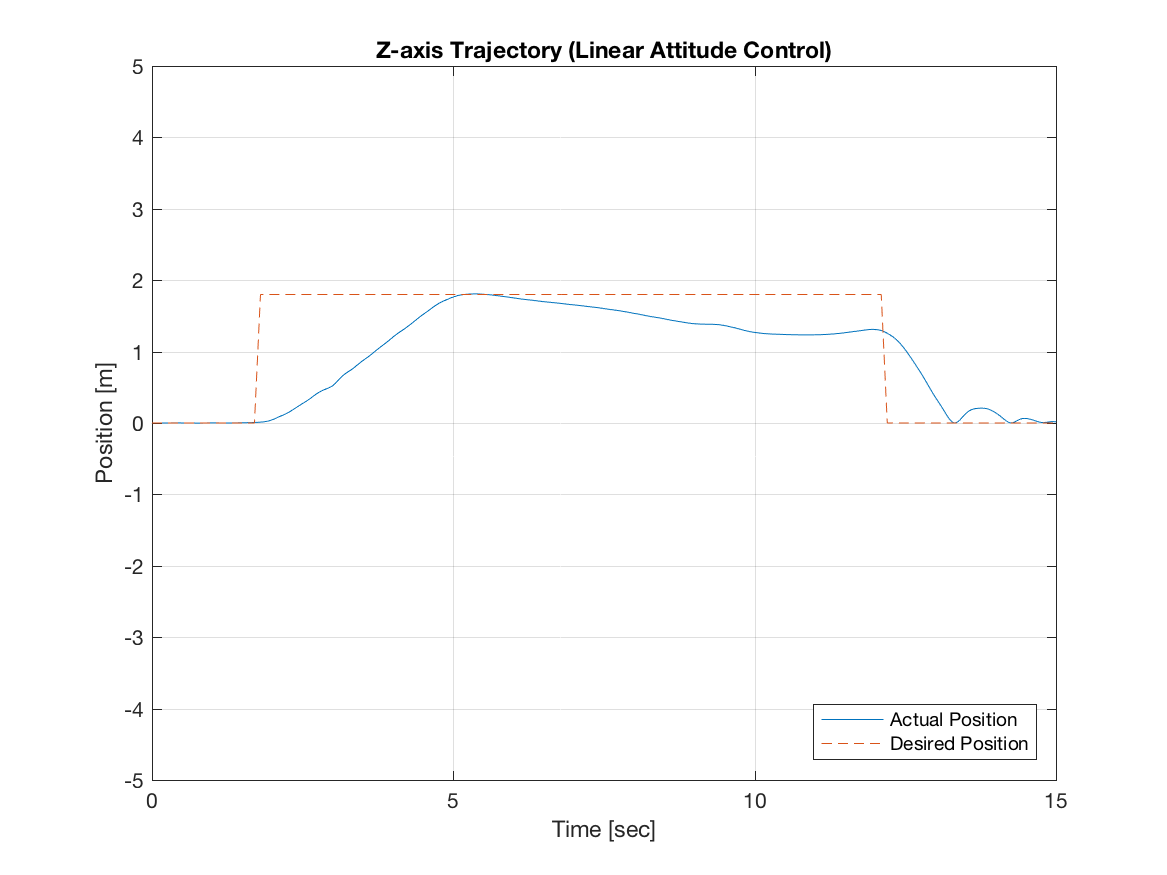
\includegraphics[width=0.45\textwidth]{graphics/experiment_plots/pitch_minus_pid_position_z.png}

    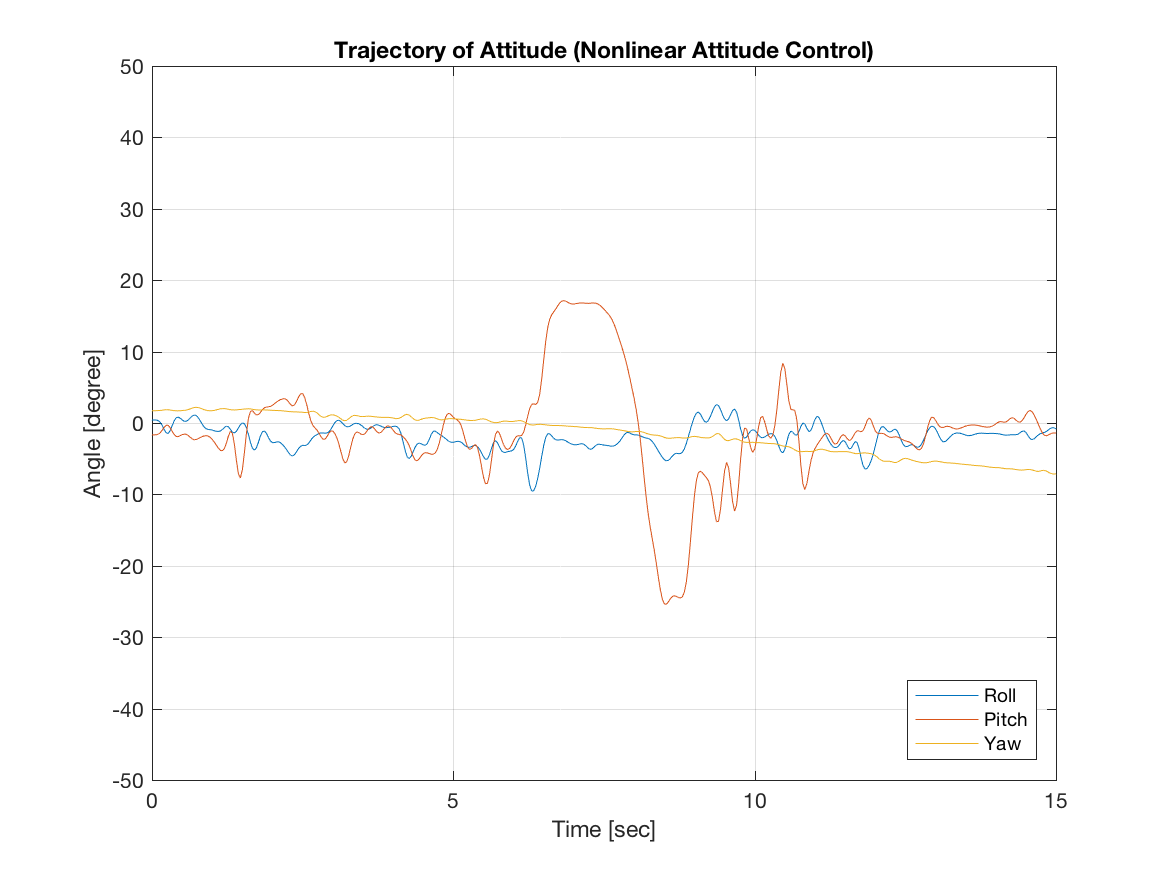
\includegraphics[width=0.45\textwidth]{graphics/experiment_plots/pitch_minus_non_attitude.png}
    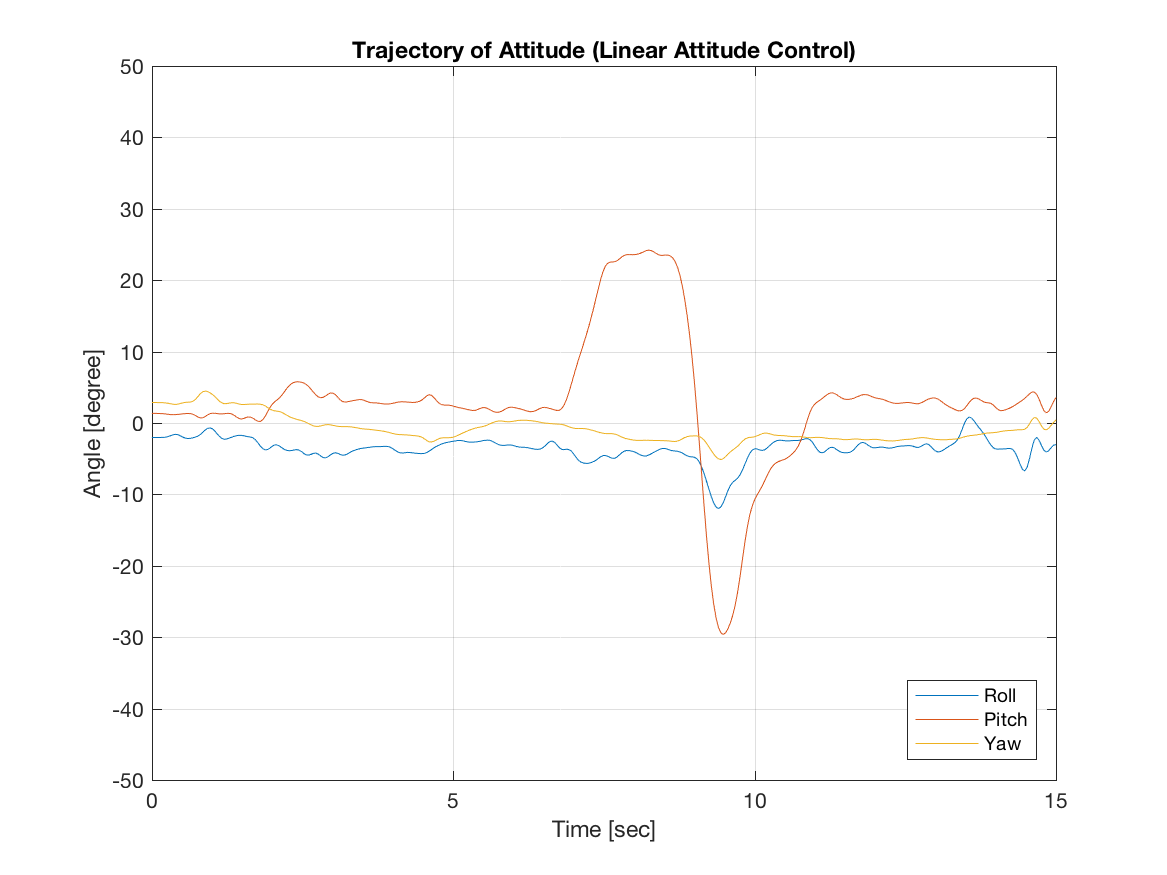
\includegraphics[width=0.45\textwidth]{graphics/experiment_plots/pitch_minus_pid_attitude.png}
    \caption{Experiment Result (Case 5)}
    \label{fig:exp_pitch_minus}
\end{figure}

\begin{figure}
    \centering
    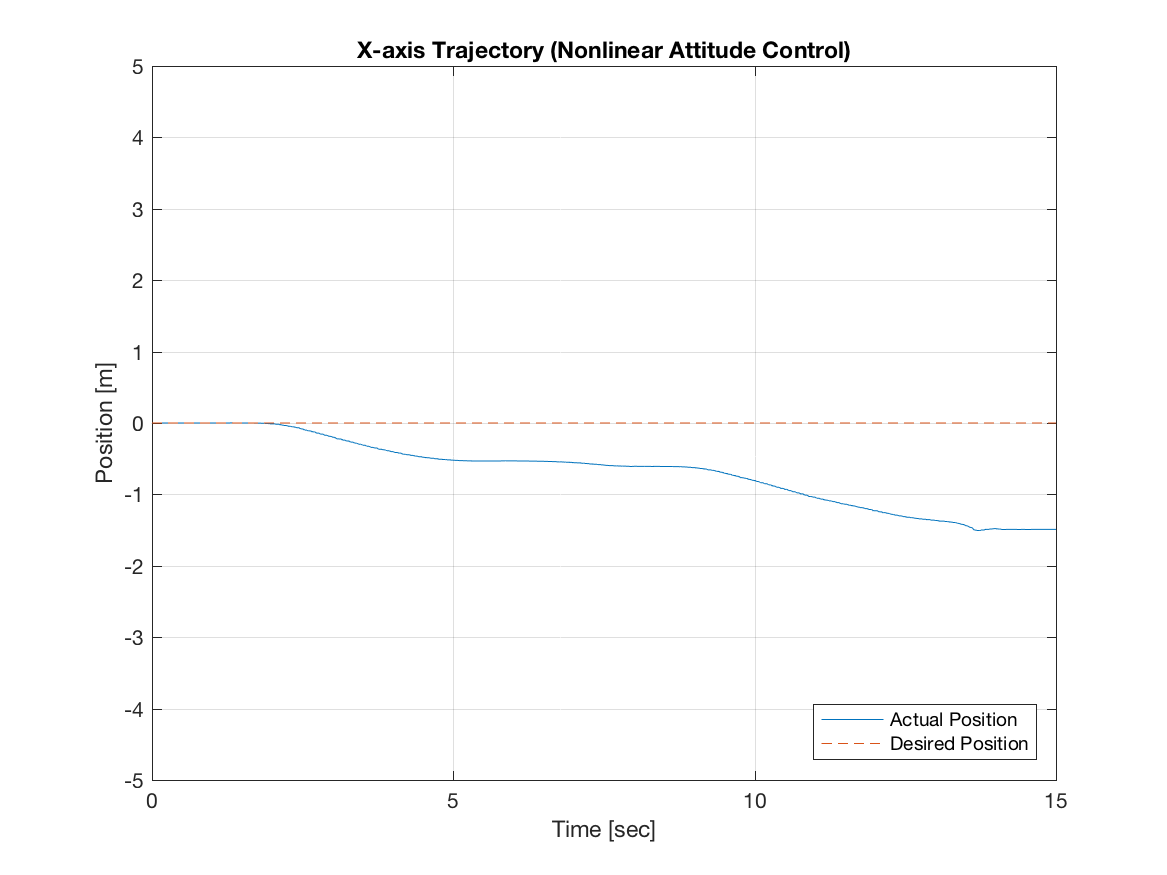
\includegraphics[width=0.45\textwidth]{graphics/experiment_plots/yaw_plus_non_position_x.png}
    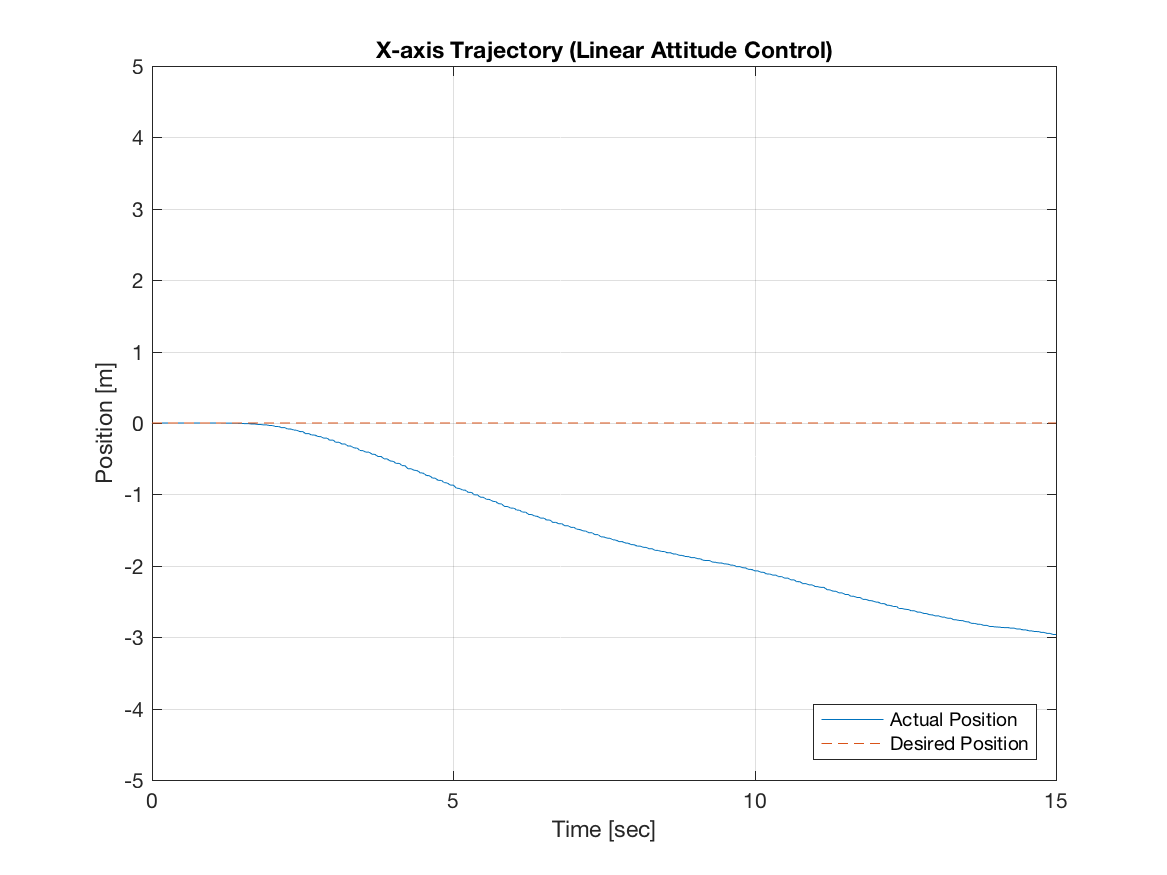
\includegraphics[width=0.45\textwidth]{graphics/experiment_plots/yaw_plus_pid_position_x.png}
    
    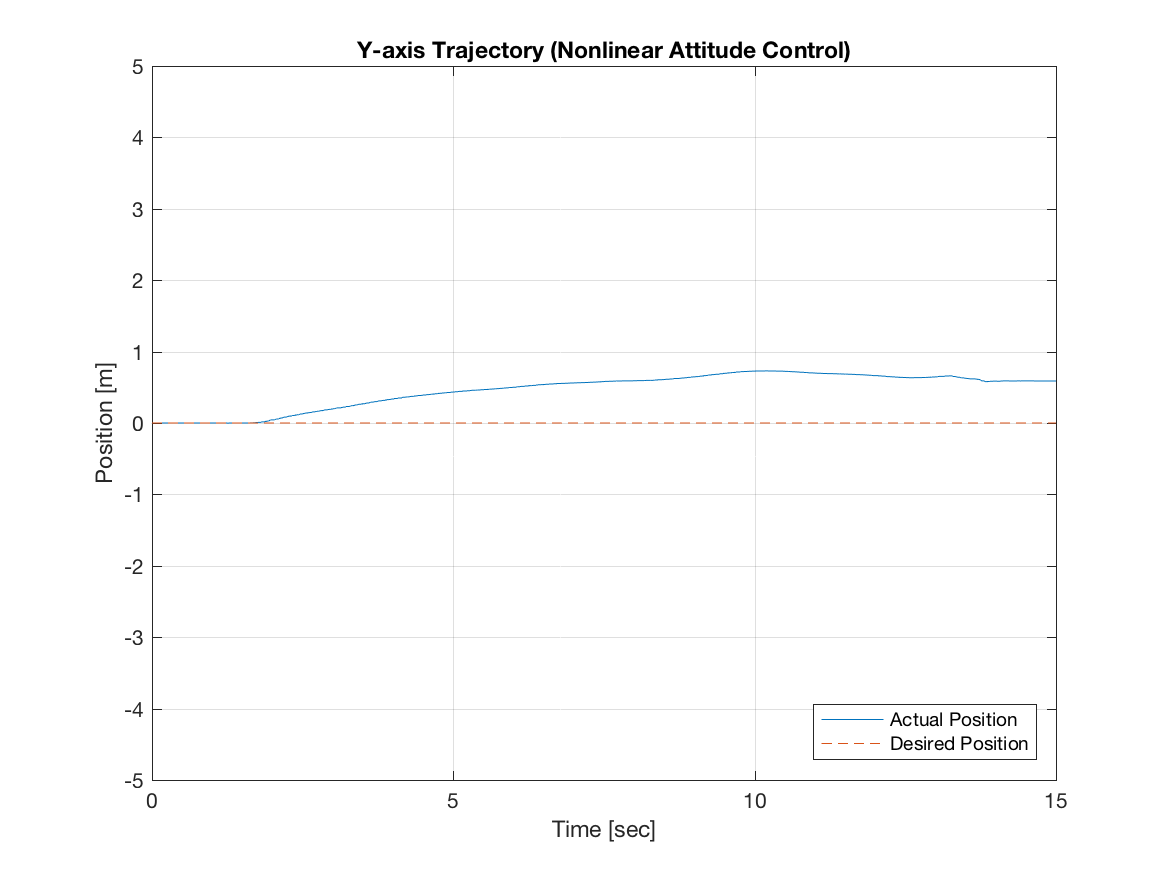
\includegraphics[width=0.45\textwidth]{graphics/experiment_plots/yaw_plus_non_position_y.png}
    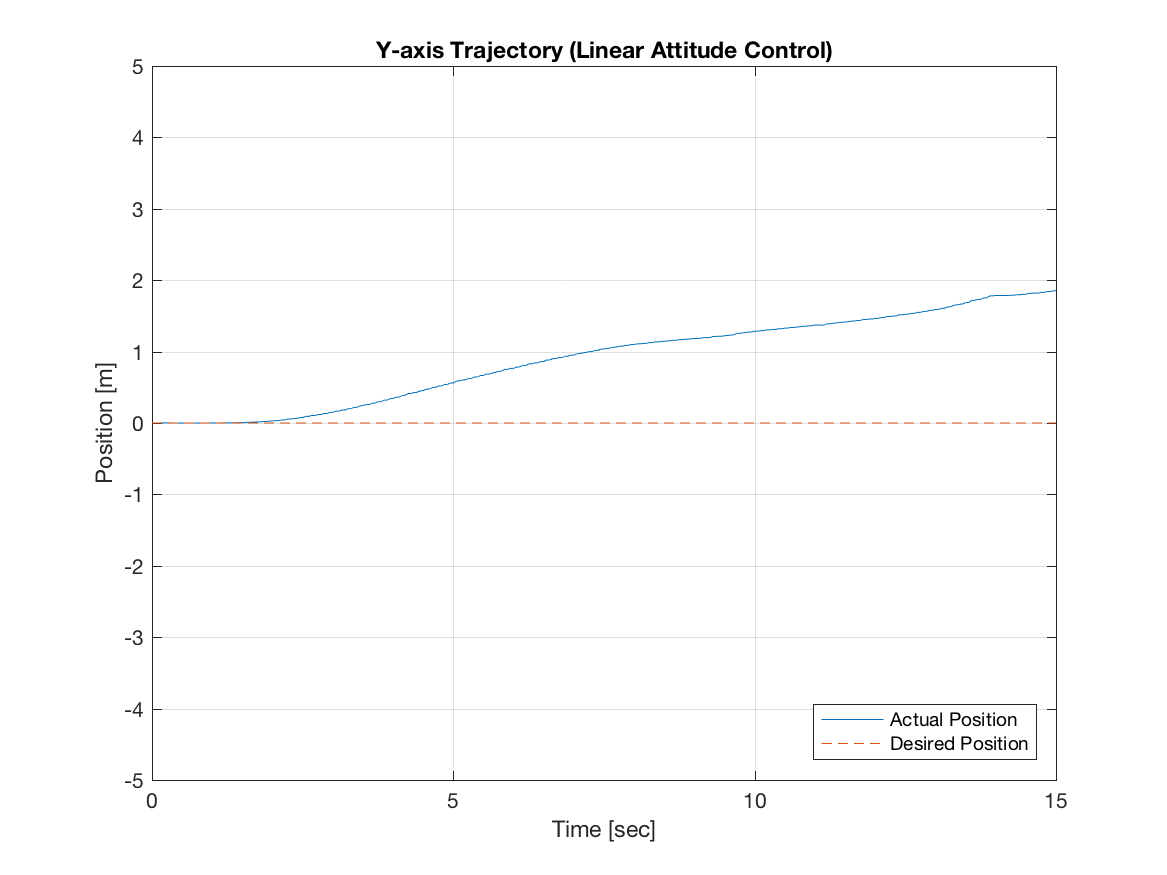
\includegraphics[width=0.45\textwidth]{graphics/experiment_plots/yaw_plus_pid_position_y.png}
    
    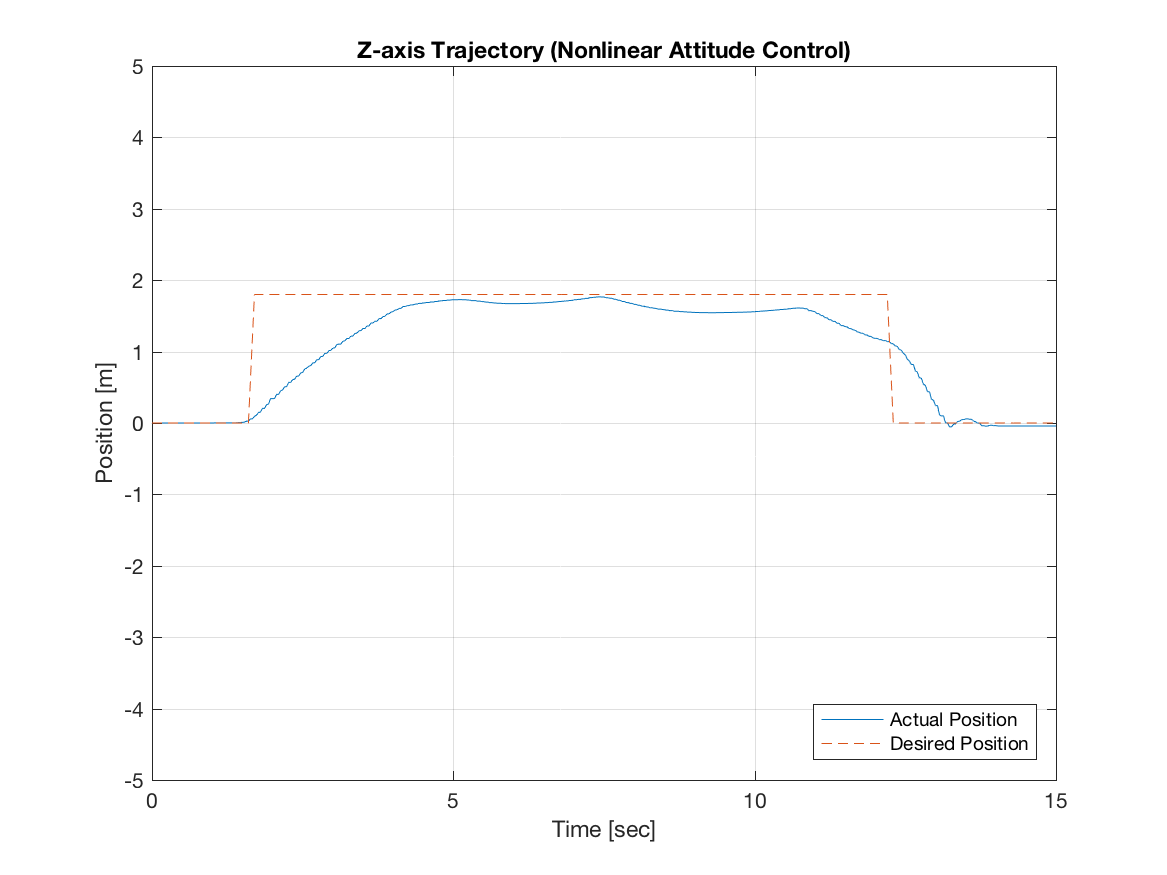
\includegraphics[width=0.45\textwidth]{graphics/experiment_plots/yaw_plus_non_position_z.png}
    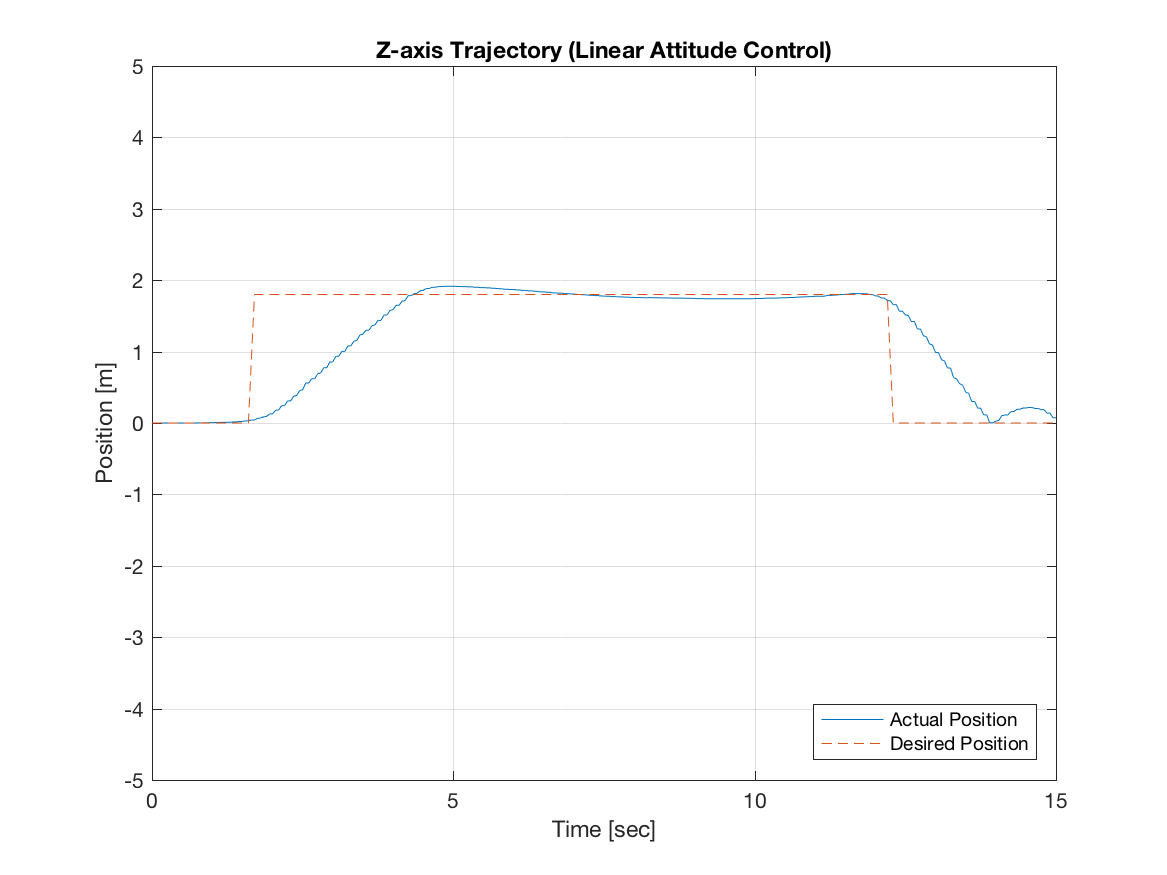
\includegraphics[width=0.45\textwidth]{graphics/experiment_plots/yaw_plus_pid_position_z.png}

    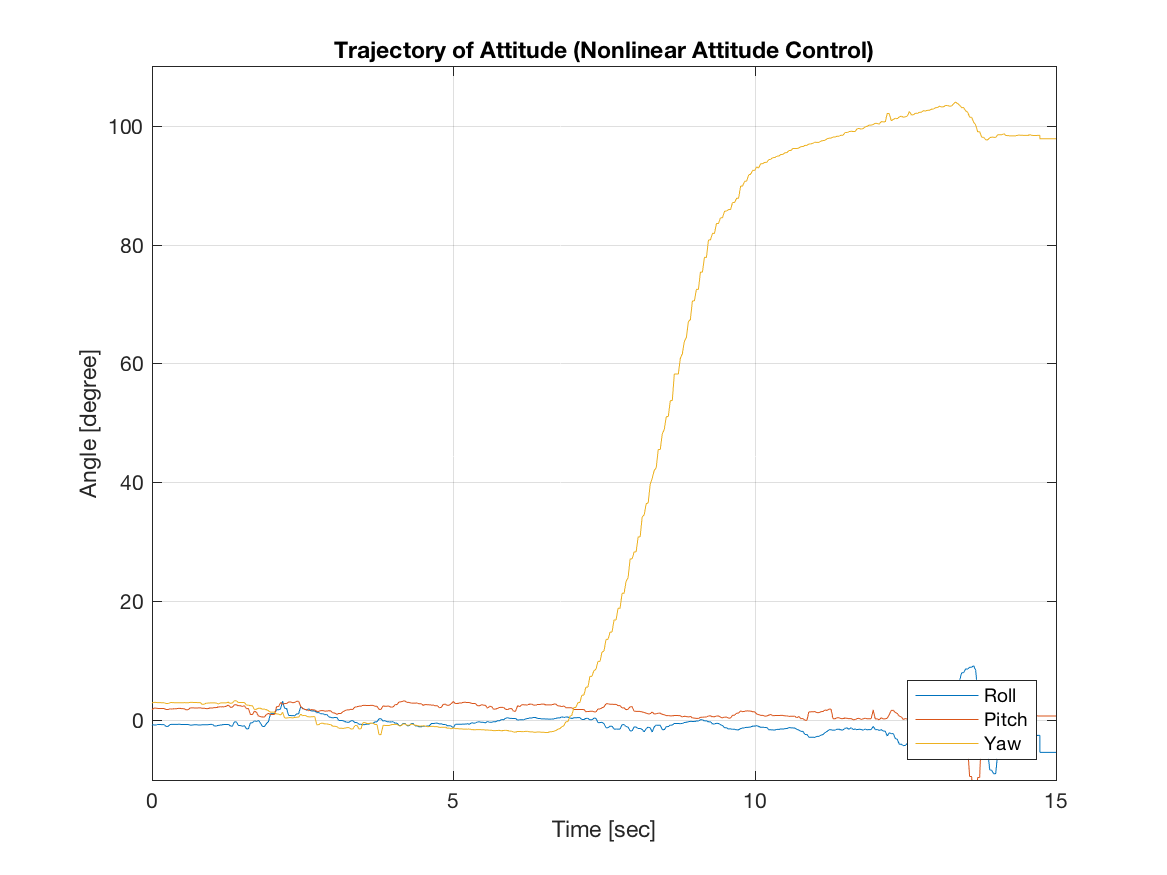
\includegraphics[width=0.45\textwidth]{graphics/experiment_plots/yaw_plus_non_attitude.png}
    \includegraphics[width=0.45\textwidth]{graphics/experiment_plots/yaw_plus_pid_attitude.png}
    \caption{Experiment Result (Case 6)}
    \label{fig:exp_yaw_plus}
\end{figure}

\begin{figure}
    \centering
    \includegraphics[width=0.45\textwidth]{graphics/experiment_plots/yaw_minus_non_position_x.png}
    \includegraphics[width=0.45\textwidth]{graphics/experiment_plots/yaw_minus_pid_position_x.png}
    
    \includegraphics[width=0.45\textwidth]{graphics/experiment_plots/yaw_minus_non_position_y.png}
    \includegraphics[width=0.45\textwidth]{graphics/experiment_plots/yaw_minus_pid_position_y.png}
    
    \includegraphics[width=0.45\textwidth]{graphics/experiment_plots/yaw_minus_non_position_z.png}
    \includegraphics[width=0.45\textwidth]{graphics/experiment_plots/yaw_minus_pid_position_z.png}

    \includegraphics[width=0.45\textwidth]{graphics/experiment_plots/yaw_minus_non_attitude.png}
    \includegraphics[width=0.45\textwidth]{graphics/experiment_plots/yaw_minus_pid_attitude.png}
    \caption{Experiment Result (Case 7)}
    \label{fig:exp_yaw_minus}
\end{figure}

\subsection{Discussion}
As discussed above, the quadrotor does not have internal position measurement of the x,y-axis directions, and therefore, there are drifts along the x,y-axis directions in every case. The position estimator uses integration of values from the internal accelerometer. Errors are accumulated by iteration, and therefore, position drifts are not avoidable. The errors caused by drifts are usually less severe with the nonlinear control system introduced in Chapter \ref{ch:control_system}. The drift occurs especially when the quadrotor takes off and lands. Dynamic factors, such as corrosion between the quadrotor's leg and the ground, are potential reasons of drifts at taking off and landing. Also, the aerodynamic model may be different near the ground and, therefore, may cause drifts as well.

In most cases, x, y-axis position errors of the linear controller are greater than the errors of the nonlinear controller. In Case 1, the y-axis drift is less than 1 m with the nonlinear control system while the error is about up to 3 m with the linear control system, and the x-axis drifts of both controllers are similar. In Cases 4 and 5, the x, y-axis position errors with the nonlinear attitude control are bounded up to 1 m, but the errors of the linear attitude control grow up to 3 m. The x, y-axis errors show similar tendencies in Cases 2 and 3. However, compared with Cases 4 and 5, the errors with the linear control system do not exceed 2 m. In Cases 6 and 7, the x, y-axis error rates of the linear control system are twice greater than the error rates of the nonlinear control system. We were not able to further reduce the position errors of the PID attitude control by tuning the gains. From these results, we can conclude that the nonlinear control system has an advantage of superior performance, compared with the linear control system.

However, the nonlinear control system does not seem to have an advantage with respect to z-axis position over an conventional PID control system. There are increasing and decreasing of altitude while the quadrotor changes its attitude, but z-axis position errors of both controllers are less than 0.5 m in most cases. As mentioned in Chapter \ref{ch:system}, the Pixhawk autopilot is equipped with an internal barometer to measure altitude and frequently corrects position estimation of double integration of acceleration. Therefore, with more precise altitude estimation, the quadrotor stabilizes its altitude better than its x,y-axis position.

In addition, time for the quadrotor to reach desired position with the nonlinear control system is approximately the same as the one with the linear attitude control since there is an upper limit of desired velocity. However, as shown in Figures \ref{fig:exp_roll_plus} - \ref{fig:exp_pitch_minus}, the quadrotor with the nonlinear control system responses fast and reaches to the maximum velocity, while it moves more smoothly with the linear control system. Also, as shown in Figures \ref{fig:exp_yaw_plus} and \ref{fig:exp_yaw_minus}, yaw control is more stabilized with the nonlinear control system. These support globally exponentially stability of the nonlinear attitude control in Section \ref{sec:inner_loop} and the results of simulation in Section \ref{sec:simulation} that the nonlinear control converges to desired attitude faster than PID attitude control does since the quadrotor's attitude affects the direction of acceleration. Therefore, we can conclude that the nonlinear control system also has an advantage of its stability.

However, the \(K_{\omega}\) and \(\Lambda\) gains should be further tuned for the nonlinear control to draw a definitive conclusion between the nonlinear control method and the PID attitude controller method. Also, there are constant yaw drifts at both control systems in Cases 2 and 3, Yaw angle increases when the quadrotor moves to right, while the yaw angle decreases when the quadrotor moves to the left. We can presume that the misalignment of the internal gyroscope or the different output curves of the DC motors caused the drifts.